%%%%%%%%%%%%%%%%%%%%%%%%%%%%%%%%%%%%%%%%%%%%%%%%%%%%%%%%%%%%%%%%%%%%%%%%%%%%%%%%%%%%%%%%%
% Khóa luận tốt nghiệp/Tiểu luận 
% LaTeX Template
% Phiên bản 1.0 (tạo ra ngày 05/10/2022)
%
% Template này có thể được download tại:
% https://github.com/cpc1996/HUS-Dissertation-Template
%
% Phiên bản 1.0 được chỉnh sửa bởi:
% Công Phương Cao (congphuongcao_t59@hus.edu.vn)
% Nguyễn Cảnh Việt (vietncp@gmail.com)
% Nguyễn Tiến Cường (ngtiencuong@gmail.com)
%
% Template được tham khảo từ một phiên bản template của:
% Steve Gunn (http://users.ecs.soton.ac.uk/srg/softwaretools/document/templates/)
% Sunil Patel (http://www.sunilpatel.co.uk/thesis-template/)
%
%%%%%%%%%%%%%%%%%%%%%%%%%%%%%%%%%%%%%%%%%%%%%%%%%%%%%%%%%%%%%%%%%%%%%%%%%%%%%%%%%%%%%%%%%


%----------------------------------------------------------------------------------------
%	(KHÔNG CHỈNH SỬA PHẦN NÀY)
%
%	PHẦN 1: CÁC PACKAGE CƠ BẢN VÀ CÁC TÙY CHỈNH VĂN BẢN
%----------------------------------------------------------------------------------------

\documentclass[
12pt,
oneside,
english,
doublespacing,
nolistspacing,
liststotoc,
parskip,
headsepline,
chapterinoneline,
]{MastersDoctoralThesis}

% \usepackage[utf8]{inputenc} 
\usepackage[utf8]{vietnam} 
%\usepackage[T1]{fontenc}

\usepackage{mathptmx}
\usepackage{amsmath}
\allowdisplaybreaks

%https://www.overleaf.com/learn/latex/Biblatex_citation_styles
%\usepackage[backend=bibtex,style=authoryear,natbib=true]{biblatex}
\usepackage[backend=bibtex,style=numeric,citestyle=ieee,natbib=true]{biblatex}

\addbibresource{main.bib}

\usepackage[autostyle=true]{csquotes}


%----------------------------------------------------------------------------------------
%	PHẦN 2: CÁC PACKAGE BỔ TRỢ THÊM VÀO TRONG QUÁ TRÌNH BIÊN SOẠN
%----------------------------------------------------------------------------------------

\usepackage{multirow}
\usepackage{subfigure}
\usepackage[fontsize=13pt]{scrextend}

%https://www.sascha-frank.com/latex-font-size.html
%https://tex.stackexchange.com/questions/103286/how-to-change-section-subsection-font-size
\usepackage{titlesec}

\titleformat{\section}
{\normalfont\fontsize{13}{13}\bfseries}{\thesection}{1em}{}

\titleformat{\subsection}
{\normalfont\fontsize{13}{13}\bfseries\itshape}{\thesubsection}{1em}{}

\usepackage{listings} 		% Liệt kê/trích dẫn code

%https://tex.stackexchange.com/questions/351961/how-to-indent-code-in-beginverbatim
\usepackage{fancyvrb} 		% Fancy Verbatim
\fvset{tabsize=4,vspace=0pt,fontsize=\footnotesize}

\usepackage{longtable} 		% Bảng dài - Long table

\usepackage[figuresright]{rotating} % Bảng ngang - Sideways table
\usepackage{tabularx}

\usepackage{fontawesome5} 	% Các biểu tượng, ký hiệu đặc biệt

\usepackage{tikz} 			% Vẽ hình
\usetikzlibrary{calc}


%----------------------------------------------------------------------------------------
%	(KHÔNG CHỈNH SỬA PHẦN NÀY)
%
%	PHẦN 3: CÁC TÙY CHỈNH LIỆT KÊ SOURCE CODE 
%----------------------------------------------------------------------------------------

%https://tex.stackexchange.com/questions/33039/using-ttfamily-with-bfseries-or-how-to-enable-bold-in-fixed-width-font
\renewcommand{\ttdefault}{pcr}
\newenvironment{pcr}{\fontfamily{pcr}\selectfont}

\definecolor{backcolor}{HTML}{f5fffc}
\definecolor{darkpink}{rgb}{0.75,0.25,0.5}
\definecolor{cadetblue}{rgb}{.6,.8,.8}

\lstset{
	tabsize			= 4,
	breaklines		= true,
	basicstyle		= \ttfamily\color{black}\bfseries\scriptsize,
	identifierstyle	= \ttfamily\color{black},
	keywordstyle	= \ttfamily\color{blue}\bfseries,  
	stringstyle		= \ttfamily\color{Red},
	commentstyle	= \itshape\color{cyan},
	%===================================================================================
	frame			= l,
	numbers			= left,
	stepnumber		= 1, 
	upquote			= true,
	numberstyle		= \tiny\color{Gray},
	backgroundcolor	= \color{backcolor},
	rulecolor		= \color{lightgray},
	rulesepcolor	= \color{lightgray},
	showstringspaces=false
	keepspaces		= true, 
	belowcaptionskip= 1\baselineskip,
	xleftmargin		= \parindent,
	%	escapeinside	= {@}{@},
	numbersep		= 7pt
}

\lstdefinestyle{codeC} {
	%https://www.pvv.ntnu.no/~berland/latex/docs/listings.pdf
	%https://www.overleaf.com/learn/latex/Using_colours_in_LaTeX
	language		= [ISO]C++, 
	basicstyle		= \linespread{1.0}\ttfamily\color{black}\bfseries\scriptsize,
	identifierstyle	= \ttfamily\color{black},
	keywordstyle	= \ttfamily\color{blue}\bfseries,  
	stringstyle		= \ttfamily\color{Red},
	commentstyle	= \itshape\color{cyan}, 
	morekeywords	= {FILE},
	%	emphstyle		= \ttfamily\color{red}\bfseries,
	%	emph			= { auto,break,case,char,const,continue,default,do,double,else,enum,extern,float,for,goto,if,int,long,register,return,short,signed,sizeof,static,struct,switch,typedef,union,unsigned,void,volatile,while,FILE},
	%https://tex.stackexchange.com/questions/283170/using-different-colors-for-different-keywords-in-lstlisting
	classoffset		= 1, % starting new class
	otherkeywords	= {\#include},
	morekeywords	= {\#include},
	keywordstyle	= \ttfamily\color{Green}\bfseries,
	morecomment		= [s][\bfseries\color{Orange}]{<a}{>},% a b d e f i l m n q r s t u v
	morecomment		= [s][\bfseries\color{Orange}]{<b}{>},
	morecomment		= [s][\bfseries\color{Orange}]{<d}{>},
	morecomment		= [s][\bfseries\color{Orange}]{<e}{>},
	morecomment		= [s][\bfseries\color{Orange}]{<f}{>},
	morecomment		= [s][\bfseries\color{Orange}]{<i}{>},
	morecomment		= [s][\bfseries\color{Orange}]{<l}{>},
	morecomment		= [s][\bfseries\color{Orange}]{<m}{>},
	morecomment		= [s][\bfseries\color{Orange}]{<n}{>},
	morecomment		= [s][\bfseries\color{Orange}]{<q}{>},
	morecomment		= [s][\bfseries\color{Orange}]{<r}{>},
	morecomment		= [s][\bfseries\color{Orange}]{<s}{>},
	morecomment		= [s][\bfseries\color{Orange}]{<t}{>},
	morecomment		= [s][\bfseries\color{Orange}]{<u}{>},
	morecomment		= [s][\bfseries\color{Orange}]{<v}{>},
	morecomment		= [l][\bfseries\color{Green}]{\#define},
	classoffset		= 0,
}

\lstdefinestyle{plaintext} {
	%https://www.pvv.ntnu.no/~berland/latex/docs/listings.pdf
	%https://www.overleaf.com/learn/latex/Using_colours_in_LaTeX
	language		= bash, 
	basicstyle		= \linespread{1.0}\ttfamily\color{black}\bfseries\scriptsize,
	identifierstyle	= \ttfamily\color{black},
	keywordstyle	= \ttfamily\color{black}\bfseries,  
	stringstyle		= \ttfamily\color{black},
	commentstyle	= \itshape\color{gray}, 
	%	showspaces		= true,
	%	showstringspaces= true,
	showtabs		= true,
	tab				= \textcolor{lightgray}{$\to$},
%	literate=*
%	{0}{{{\color{darkpink}0}}}{1}
}

\lstdefinestyle{codeMatlab} {
	language		= Matlab,
	basicstyle		= \linespread{1.0}\ttfamily\color{black}\bfseries\scriptsize,
	identifierstyle	= \ttfamily\color{black},
	keywordstyle	= \ttfamily\color{blue}\bfseries,  
	stringstyle		= \ttfamily\color{magenta},
	commentstyle	= \itshape\color{LimeGreen},
	morecomment		= [l][\bfseries\color{red}]{\%\%},
	morekeywords	= {syms,switch,case,otherwise,ones,class,inline,vectorize,factorial,xlim,ylim,ezplot,pie,ezmesh,ezsurf,ezcontour,ezplot3,solve,double,subs,fsolve,fminsearch,compose,jacobian,int,dblquad,triplequad,limit,finverse,simplify,taylor,symsum,evalin,symengine,matlabFunction,poly2sym,lsqcurvefit,ppval,dsolve},
	literate		=*,
	literate		=*
	{^}{\textasciicircum}{1}
}

\lstdefinestyle{codePython} {
	language		= Python,
	basicstyle		= \linespread{1.0}\ttfamily\color{black}\bfseries\scriptsize,
	identifierstyle	= \ttfamily\color{black},
	keywordstyle	= \ttfamily\color{blue}\bfseries,  
	stringstyle		= \ttfamily\color{LimeGreen},
	commentstyle	= \itshape\color{cadetblue},
	morekeywords	= {self},
	emph			={MyClass,__init__},
	emphstyle		=\ttb\color{red},
	literate		=*,
	literate		=*
	{^}{\textasciicircum}{1}
}

%https://www.alanshawn.com/tech/2019/09/01/emulate-terminal.html
\definecolor{tergreen}{rgb}{0,0.6,0}
\definecolor{tergray}{rgb}{0.5,0.5,0.5}
\definecolor{termauve}{rgb}{0.58,0,0.82}
\definecolor{terminalbgcolor}{HTML}{330033}
\definecolor{terminalrulecolor}{HTML}{000099}
\lstdefinestyle{console} {
	backgroundcolor	= \color{terminalbgcolor},
	basicstyle		= \linespread{1.0}\ttfamily\color{white}\bfseries\scriptsize,
	identifierstyle	= \ttfamily\color{white}\bfseries\scriptsize,
	breakatwhitespace=false,
	breaklines		= true,
	captionpos		= b,
	commentstyle	= \color{tergreen},
	deletekeywords	= {...},
	escapeinside	= {\%*}{*)},
	extendedchars	= true,
	frame			= single,
	keepspaces		= true,
	keywordstyle	= \color{blue},
	language		= {},
	morekeywords	= {*,...},
	numbers			= none,
	numbersep		= 5pt,
	framerule		= 2pt,
	numberstyle		= \color{tergray}\tiny\selectfont,
	rulecolor		= \color{terminalrulecolor},
	showspaces		= false,
	showstringspaces= false,
	showtabs		= false,
	stepnumber		= 2,
	stringstyle		= \color{termauve},
	tabsize			= 2,
	literate		=*
}


%----------------------------------------------------------------------------------------
%	(KHÔNG CHỈNH SỬA PHẦN NÀY)
%
%	PHẦN 4: CÁC TÙY CHỈNH KHỔ GIẤY VÀ CĂN LỀ
%----------------------------------------------------------------------------------------

\geometry{
	paper=a4paper,
	inner=3cm,
	outer=2cm,
	bindingoffset=0cm,
	top=0.6cm,
	bottom=2.0cm,
}


%----------------------------------------------------------------------------------------
%	PHẦN 5: THÔNG TIN VỀ Khóa luận tốt nghiệp/Tiểu luận (THESIS INFORMATION)
%----------------------------------------------------------------------------------------

\author{Nguyễn Trường Danh} 			% Ví dụ: "Nguyễn Thị Thu Thảo"
\thesistitle{Neural Structured Learning with Python/TensorFlow} % Ví dụ: "Nghiên cứu chế tạo và tính chất quang học của vật liệu nano LaF3:Sm3+"

\supervisor {TS. NGUYỄN TIẾN CƯỜNG} 	% Ví dụ: "PGS. TS. Nguyễn Ngọc Long"
\supervisorr{} 	% Tên này nếu không có thì để trống!

\field{NGÀNH KỸ THUẬT ĐIỆN TỬ VÀ TIN HỌC} 					% Ví dụ: "Ngành Vật lý", "Ngành Hóa học", v.v.
\program{CHƯƠNG TRÌNH ĐÀO TẠO CHUẨN} 			% Ví dụ: "Chương trình đào tạo chuẩn", "Chương trình đào tạo cử nhân tài năng", v.v.
\doctype{TIỂU LUẬN} % Điền vào đây: "Khóa luận tốt nghiệp đại học hệ chính quy" hoặc "Tiểu luận"

\university{\href{http://hus.vnu.edu.vn}{Trường Đại học Khoa học Tự nhiên}}
\department{\href{http://hus.vnu.edu.vn/gioi-thieu/co-cau-to-chuc/khoa-truc-thuoc/khoa-vat-ly.html}{Khoa Vật lý}}

\AtBeginDocument{
	\hypersetup{pdftitle=\ttitle}
	\hypersetup{pdfauthor=\authorname}
}


\begin{document}

\lstset{style=codeC}	% Thiết lập ngôn ngữ C/C++ là ngôn ngữ mặc định cho phần liệt kê souce code của cả bài

\frontmatter 			% Sử dụng hệ thống đánh số La Mã (i, ii, iii, iv...) cho những trang trước phần mục lục

\pagestyle{plain} 


%----------------------------------------------------------------------------------------
%	(KHÔNG CHỈNH SỬA PHẦN NÀY)
%
%	Phần 6: TRANG TIÊU ĐỀ/TRANG BÌA (TITLE PAGE)
%----------------------------------------------------------------------------------------

% TRANG BÌA:
\begin{titlepage}
	\begin{tikzpicture}[overlay,remember picture]
		\draw [line width=3pt]
		($ (current page.north west) + (2.0cm,-2.0cm) $)
		rectangle
		($ (current page.south east) + (-1.5cm,1.8cm) $);
		\draw [line width=1pt]
		($ (current page.north west) + (2.15cm,-2.15cm) $)
		rectangle
		($ (current page.south east) + (-1.65cm,1.95cm) $); 
	\end{tikzpicture}
	\begin{center}
		
		\vspace{-.04\textheight}
		\noindent\scshape
		\large \, \href{https://www.vnu.edu.vn/home/}{ĐẠI HỌC QUỐC GIA HÀ NỘI}\\
		\vspace{-0.25cm}{\large \MakeUppercase \univname}\\
		\vspace{-0.25cm}{\large \bfseries \MakeUppercase \deptname}\\[0.5cm]
		
\includegraphics{Logo/Logo_HUS_notext_nocolor}
		
		\vspace{1.0cm}
		
		{\large \MakeUppercase \authorname}
		
		\vspace{2.5cm}
		
		{\Large \bfseries \MakeUppercase\ttitle\par}
		
		\vspace{2.5cm}
		
		{\normalsize \docname\\ \fieldname\\ (\progname)\\}
	
		\vfill
		
		\textbf{Hà Nội - \the\year{}}
	\end{center}
\end{titlepage}


% TRANG BÌA LÓT:
\begin{titlepage}
	\begin{tikzpicture}[overlay,remember picture]
		\draw [line width=3pt]
		($ (current page.north west) + (2.0cm,-2.0cm) $)
		rectangle
		($ (current page.south east) + (-1.5cm,1.8cm) $);
		\draw [line width=1pt]
		($ (current page.north west) + (2.15cm,-2.15cm) $)
		rectangle
		($ (current page.south east) + (-1.65cm,1.95cm) $); 
	\end{tikzpicture}
	\begin{center}
		
		\vspace{-.04\textheight}
		\noindent\scshape
		\large \, \href{https://www.vnu.edu.vn/home/}{ĐẠI HỌC QUỐC GIA HÀ NỘI}\\
		\vspace{-0.25cm}{\large \MakeUppercase \univname}\\
		\vspace{-0.25cm}{\large \bfseries \MakeUppercase \deptname}\\[0.5cm]
		
\includegraphics{Logo/Logo_HUS_notext}
		
		\vspace{1.0cm}
		
		{\large \MakeUppercase \authorname}
		
		\vspace{2.5cm}
		
		{\Large \bfseries \MakeUppercase\ttitle\par}
		
		\vspace{2.5cm}
		
		{\normalsize \docname\\ \fieldname\\ (\progname)\\}
	 
	 	\vspace{2.5cm}
	 	
		\begin{minipage}[t]{0.49\textwidth}
			\begin{flushright} \large \bfseries
				giảng viên hướng dẫn:\;
			\end{flushright}
		\end{minipage}
		\begin{minipage}[t]{0.5\textwidth}
			\begin{flushleft} \large \bfseries
				\supname\\
				\supnamee
			\end{flushleft}
		\end{minipage}
	
		\vfill
		
		\textbf{Hà Nội - \the\year{}}
	\end{center}
\end{titlepage}


%----------------------------------------------------------------------------------------
%	Phần 7: DANH NGÔN (QUOTES)
%----------------------------------------------------------------------------------------

\vspace*{0.2\textheight}

\noindent\enquote{\itshape 
	Cái tôi và sự hiểu biết tỷ lệ nghịch với nhau. Hiểu biết càng nhiều cái tôi càng bé. Hiểu biết càng ít, cái tôi càng to.
}\bigbreak

\hfill Albert Einstein


%----------------------------------------------------------------------------------------
%	Phần 8: LỜI CẢM ƠN (ACKNOWLEDGEMENTS)
%----------------------------------------------------------------------------------------

\begin{acknowledgements}
	\addchaptertocentry{\acknowledgementname}
	\thispagestyle{empty}
	Để hoàn thành học phần cũng như báo cáo này đã có sự hướng dẫn và giúp đỡ tận tình của thầy
	TS. Nguyễn Tiến Cường. Vì vậy em muốn gửi lời cảm ơn sâu sắc nhất tới thầy đã hướng dẫn và chỉ dạy
	em tận tình trong học phần này cũng như các học phần trước. Em hi vọng sẽ được tiếp tục làm việc và học hỏi từ thầy
	và các thầy cô khác trong bộ môn ở những học phần tiếp theo, đặc biệt là khóa luận tốt nghiệp!

	% ký tên ở góc phải

	\vspace{1.5cm}
	\begin{flushright}
		\textbf{Hà Nội, \today}\\
	\end{flushright}
		% lùi tên vào giữa
		\hspace{12cm}
		Ký tên \\
		\vspace{1cm}

		\hspace{10.5cm}
		\textbf{\authorname}\\



\end{acknowledgements}


%----------------------------------------------------------------------------------------
%	(KHÔNG CHỈNH SỬA PHẦN NÀY)
%
%	Phần 9: MỤC LỤC (LIST OF CONTENTS/FIGURES/TABLES PAGES)
%----------------------------------------------------------------------------------------

\begin{spacing}{1.15}
	\tableofcontents 	% In ra mục lục chính
\end{spacing}

\begin{spacing}{1.15}
	\listoffigures 		% In ra danh sách hình vẽ
\end{spacing}

%\begin{spacing}{1.15}
%	\listoftables		% In ra danh sách bảng
%\end{spacing}


%----------------------------------------------------------------------------------------
%	Phần 10: DANH SÁCH TÊN VIẾT TẮT (ABBREVIATIONS)
%----------------------------------------------------------------------------------------

\begin{abbreviations}{ll} % Thêm danh sách tên viết tắt (dưới dạng một bảng có 2 cột)

\textbf{NSL} & \textbf{N}eural \textbf{S}truct \textbf{L}earning\\
\textbf{CPU} & \textbf{C}enter \textbf{P}rocessing \textbf{U}nit\\
\textbf{GPU} & \textbf{G}raphics \textbf{P}rocessing \textbf{U}nit\\
\textbf{API} & \textbf{A}pplication \textbf{P}rogramming \textbf{I}nterface\\

\end{abbreviations}


%----------------------------------------------------------------------------------------
%	Phần 12: DANH SÁCH KÝ HIỆU (SYMBOLS)
%----------------------------------------------------------------------------------------

\begin{symbols}{lll} % Thêm danh sách các ký hiệu (dưới dạng một bảng có 3 cột)

%   Ký hiệu	& Ý nghĩa		& Đơn vị \\
	%$a$		& khoảng cách	& \si{\meter} \\
	%$P$		& công suất		& \si{\watt} (\si{\joule\per\second}) \\

	\addlinespace % Khoảng cách để phân biệt giữa ký hiệu Latin với ký hiệu La Mã

	%$\omega$ & tần số góc	& \si{\radian} \\

	
	$v_t$ & tổng bình phương của gradien trong quá khứ\\
	$\beta$ &  tham số trung bình\\
	$\alpha$ & tốc độ học\\
	$\delta L$ &  đạo hàm của hàm mất mát\\
	$w_t$ &  trọng số tại thời điểm t\\
	$w_{t-1}$ &  trọng số tại thời điểm t-1\\
	$\epsilon$ &  một hằng số dương rất nhỏ để tránh chia cho 0\\
	$\delta w_t$ &  đạo hàm của trọng số tại thời điểm t \\
	$m_t$ &  tổng các gradient tại thời điểm t.\\


		

\end{symbols}


%----------------------------------------------------------------------------------------
%	(KHÔNG CHỈNH SỬA PHẦN NÀY)
%
%	Phần 13: LỜI ĐỀ TẶNG (DEDICATION)
%----------------------------------------------------------------------------------------

%\dedicatory{Dành tặng/Dành cho/Gửi tới\ldots} 


%----------------------------------------------------------------------------------------
%	Phần 14: NỘI DUNG/CÁC CHƯƠNG Khóa luận tốt nghiệp/Tiểu luận (THESIS CONTENT - CHAPTERS)
%----------------------------------------------------------------------------------------

\mainmatter % Bắt đầu đánh số trang (1,2,3...)

\pagestyle{plain}

% Hãy thêm những chương (chapter) của khóa luận/tiểu luận vào thư mục Chapters
% Hãy bỏ chú thích những dòng nếu bạn đã bổ sung những chương vào


\chapter*{Mở đầu}


\addcontentsline{toc}{chapter}{Mở đầu}


Alan Turing, một nhà toán học lỗi lạc, người đã phá vỡ cỗ máy mã hóa Enigma của Đức quốc xã, đã đưa ra một câu hỏi làm thay đổi lịch sử, “Máy móc có thể suy nghĩ không?” vào năm 1950. Nghiên cứu thực sự bắt đầu vào năm 1956, 
tại một hội nghị được tổ chức tại Đại học Dartmouth (rất nhiều phát minh đã được đưa ra, nhờ Ivy League). Một vài người tham dự hội nghị là những người đã đưa ra ý tưởng và cũng là cái tên “Trí tuệ nhân tạo”. Nhưng vì toàn bộ 
ý tưởng là mới, mọi người đã không mua ý tưởng đó và tài trợ cho nghiên cứu sâu hơn đã bị cắt giảm. Giai đoạn này, những năm 1950 – 1980 được gọi là “AI Winter”. Tuy nhiên, vào đầu những năm 1980, chính phủ Nhật Bản đã nhìn thấy 
tương lai của AI và bắt đầu tài trợ trở lại cho lĩnh vực này. Vì điều này được kết nối với các lĩnh vực điện tử và khoa học máy tính, nên cũng có sự gia tăng đột biến trong các lĩnh vực đó. Máy AI đầu tiên được giới thiệu ra thế 
giới vào năm 1997; Deep Blue của IBM đã trở thành máy tính đầu tiên đánh bại một nhà vô địch cờ vua khi đánh bại đại kiện tướng người Nga Garry Kasparov. Ngày nay AI đóng góp hầu hết vào các lĩnh vực trong đời sống như y tế, giáo 
dục, an ninh, kinh tế và kể cả quân sự. Qua đó cho thấy được tầm quan trọng của AI.

Trong quá trình hình thành và phát triển từ những năm 50 của thế kỷ trước tới nay, có rất nhiều thư viện hay API được nghiên cứu và xây dựng để hỗ trợ cho việc phát triển AI. Trong đó có rất nhiều thư viện
khá phổ biến và mạnh mẽ như pytorch, pandas, SciPy, Keras, Theano... đặc biệt không thể thiếu thư viện TensorFlow. TensorFlow là một thư viện mã nguồn mở được phát triển bởi Google. Nó được thiết kế để
hỗ trợ việc phát triển các mô hình Machine Learning và Deep Learning. TensorFlow cũng có thể được sử dụng để phát triển các mô hình Deep Learning cho các thiết bị di động như Android và iOS. 

Một lĩnh vực khá thú vị trong AI cũng như học máy(ML) là thị giác máy tính, nghĩa là chúng ta sẽ làm cho máy tính có thể nhận biết, quan sát, và hiểu được các nội dung của các bức ảnh hoặc video. Để làm được điều đó,
chúng ta cần phải huấn luyện một mô hình học máy để nó có thể nhận biết được các đặc trưng của các bức ảnh. Trong tiểu luận này chúng ta sẽ tìm hiểu về một bài toán nhận biết chữ số viết tay với TensorFlow. Bài toán này sẽ được 
giải quyết bằng cách sử dụng thuật toán Neural Struct Learning và một mô hình mạng neural. Bài toán sử dụng bộ dữ liệu có sẵn của TensorFlow MNIST, là một bộ dữ liệu gồm các chữ số viết tay khác nhau đề huấn luyện mô hình.

Cấu trúc của bài tiểu luận này gồm ba chương:

\begin{itemize}
\item Chương 1: Tổng quan

     Ở chương này, chúng ta sẽ đi qua tổng qua về trí tuệ nhân tạo, học máy, học sâu và giới thiệu về thư viện TensorFlow.
     Ngoài ra chúng ta cũng sẽ tìm hiểu về thuật toán tối ưu Adam, thuật toán sẽ được sử dụng để huấn luyện mô hình học máy trong bài tiểu luận này.
\item Chương 2: Neural Structured Learning With Python/TensorFlow

    Ở chương này, chúng ta sẽ tìm hiểu về thuật toán Neural Structured Learning. Và khái quát bài toán cũng như sử dụng Adversarial Learning để giải quyết bài toán đề ra.

\item Chương 3: Nhận diện chữ số viết tay

    Ở chương này, chúng ta sẽ triển khai các mô hình và đào tạo nó, một mô hình cơ bản và một mô hình nâng cao sử dụng thuật toán Adversarial Learning để xem xét được ưu điểm 
    và sự khác biệt của mô hình Adversarial Learning. Sau đó chúng ta sẽ dùng hai mô hình vừa huấn luyện này để nhận biết một số các chữ số viết tay từ ảnh chụp trực tiếp.
\end{itemize}



% MỞ ĐẦU (LỜI MỞ ĐẦU - Chương 0)

\chapter*{MỞ ĐẦU} % Tên của chương
\addcontentsline{toc}{chapter}{MỞ ĐẦU} % Thêm tên chương vào mục lục

\label{Chapter0} % Để trích dẫn chương này ở chỗ nào đó trong bài, hãy sử dụng lệnh \ref{Chapter0} 

%----------------------------------------------------------------------------------------

Phần "MỞ ĐẦU" được tính là một chương nhưng không được đánh số (sử dụng lệnh \verb|\chapter*{MỞ ĐẦU}|, và được ghi ở file \texttt{\bfseries Chapters/Chapter0.tex}). Phần này sẽ giới thiệu khái quát về cấu trúc của khóa luận tốt nghiệp, những nội dung chính của các chương cũng như những lưu ý mà tác giả muốn độc giả lưu ý. Phần "MỞ ĐẦU" là một phần tùy chọn nên bạn hãy xem xét xem liệu có nên cho phần này vào khóa luận của mình không!
% Template cho một chương

\chapter{Neural Structured Learning With Python/TensorFlow} % Tên của chương

\label{Chapter2} % Thay X bằng số chương tương ứng; để trích dẫn chương này ở chỗ nào đó trong bài, hãy sử dụng lệnh \ref{ChapterX} 

%----------------------------------------------------------------------------------------
%	MỤC 1
%----------------------------------------------------------------------------------------
\newcommand{\keyword}[1]{\textbf{#1}}
\newcommand{\tabhead}[1]{\textbf{#1}}
\newcommand{\code}[1]{\texttt{#1}}
\newcommand{\file}[1]{\texttt{\bfseries#1}}
\newcommand{\option}[1]{\texttt{\itshape#1}}


\section{Neural Structured Learning}
Neural Structured Learning (NSL) là một mô hình học tập mới để huấn luyện mạng thần kinh bằng cách tận dụng các tín hiệu có cấu trúc bên cạnh các đầu vào tính 
năng. Cấu trúc có thể rõ ràng như được biểu thị bằng biểu đồ hoặc ẩn khi gây ra "nhiễu loạn đối nghich.

Các tín hiệu có cấu trúc thường được sử dụng để biểu thị các mối quan hệ hoặc sự giống nhau giữa các mẫu có thể được gắn nhãn hoặc không gắn nhãn. Do đó, việc 
tận dụng các tín hiệu này trong quá trình huấn luyện mạng thần kinh sẽ khai thác cả dữ liệu được gắn nhãn và không được gắn nhãn, điều này có thể cải thiện độ 
chính xác của mô hình, đặc biệt khi lượng dữ liệu được gắn nhãn tương đối nhỏ . Ngoài ra, các mô hình được đào tạo với các mẫu được tạo bằng cách thêm nhiễu loạn 
đối nghịch đã được chứng minh là hoạt động tốt đối với các dữ liệu không tốt được thiết kế để đánh lừa dự đoán hoặc phân loại của mô hình.

NSL khái quát hóa thành Neural Graph Learning cũng như Adversarial Learning. Khung NSL trong TensorFlow cung cấp các API và công cụ dễ sử dụng sau đây cho các 
nhà phát triển để đào tạo các mô hình với các tín hiệu có cấu trúc:
\begin{itemize}
    \item \textbf{Keras APIs} để cho phép đào tạo với đồ thị (cấu trúc rõ ràng) và nhiễu đối phương (cấu trúc ngầm định).
    \item \textbf{TF ops and functions} cho phép đào tạo với cấu trúc khi sử dụng các API TensorFlow cấp thấp hơn.
    \item \textbf{Tools} để xây dựng đồ thị và xây dựng đầu vào đồ thị để đào tạo.
\end{itemize}

\begin{figure}[h!]
    \centering
    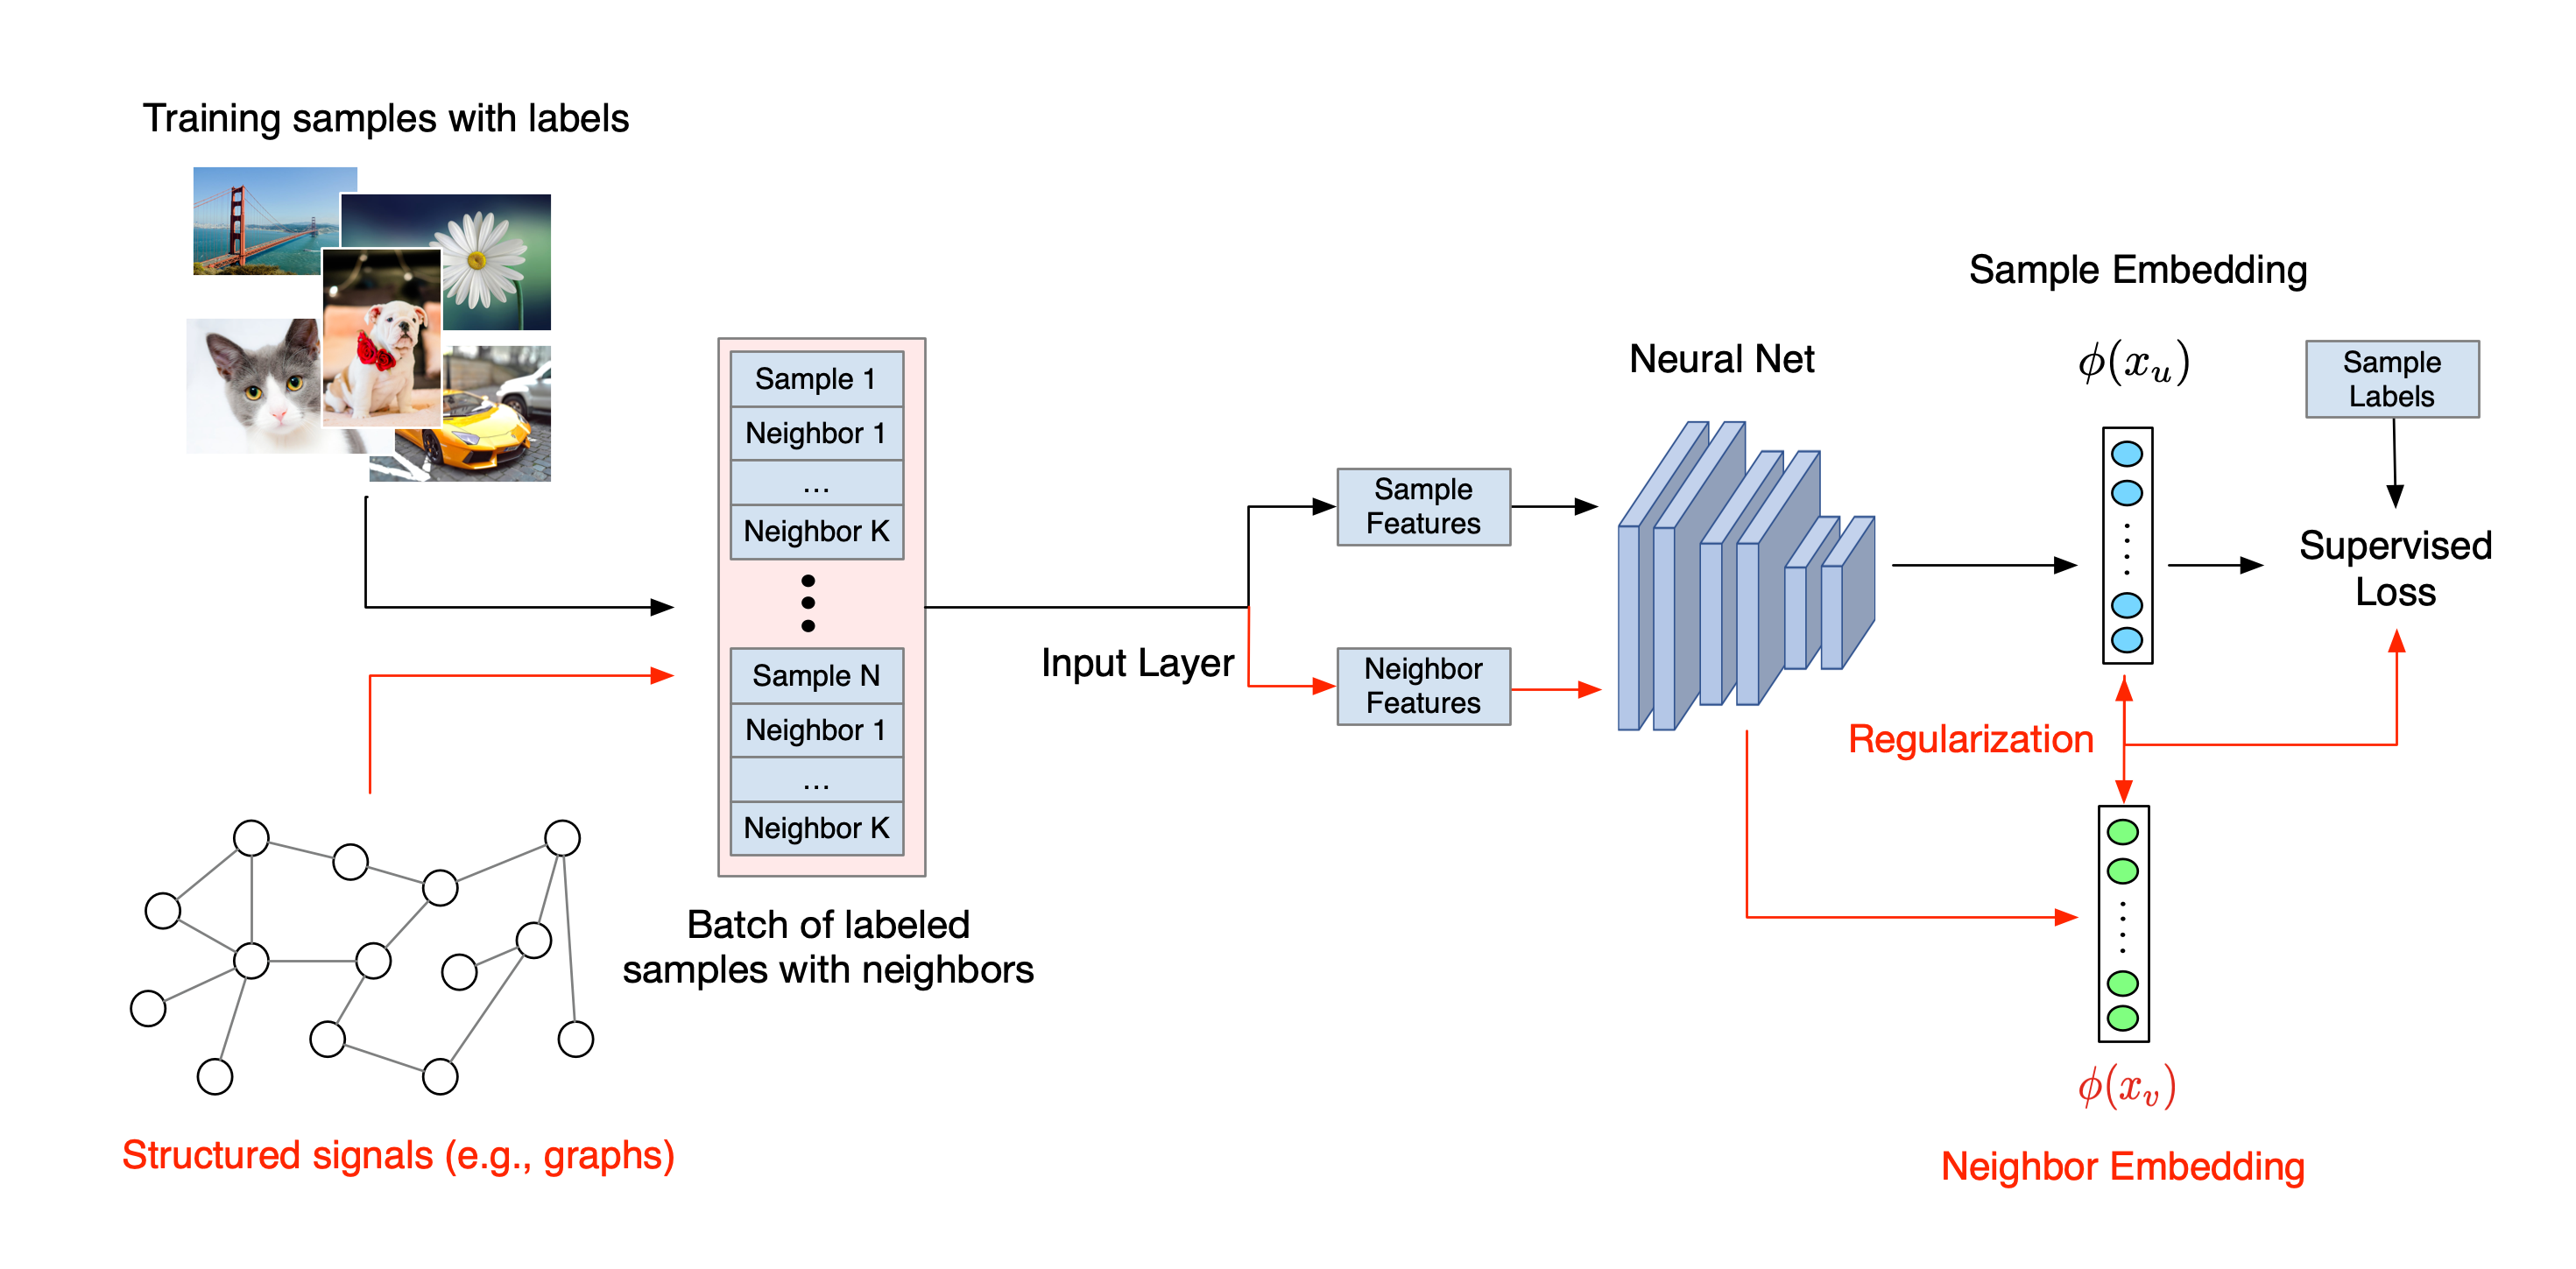
\includegraphics[width=0.8\linewidth]{Image/NSL.png}
    \caption {Neural Structured Learning}
    \label{Hình 1.2: Neural Structured Learning}
    \cite*{WEBSITE:4}
\end{figure}

Trong Neural Structured Learning (NSL), các tín hiệu có cấu trúc dù được xác định rõ ràng dưới dạng biểu đồ hay được học ngầm dưới dạng cách ví dụ đối nghịch được 
được sử dụng để thường xuyên đào tạo mạng neural, buộc mô hình phải học các dự đoán chính xác (bằng cách giảm thiểu mất mát có giám sát), đồng thời duy trì sự giống nhau giữa các đầu vào từ 
cùng một cấu trúc(bằng cách giảm thiểu tổn thất lân cận). Kỹ thuật này là chung và có thể được áp dụng trên các kiến trúc neural tùy ý, chẳng hạn như Feed-Forward NNs, CNNs, RNNs. 


\subsection{Neural Graph Learning}

\textbf{Training with natural graphs}

\begin{figure}[h!]
    \centering
    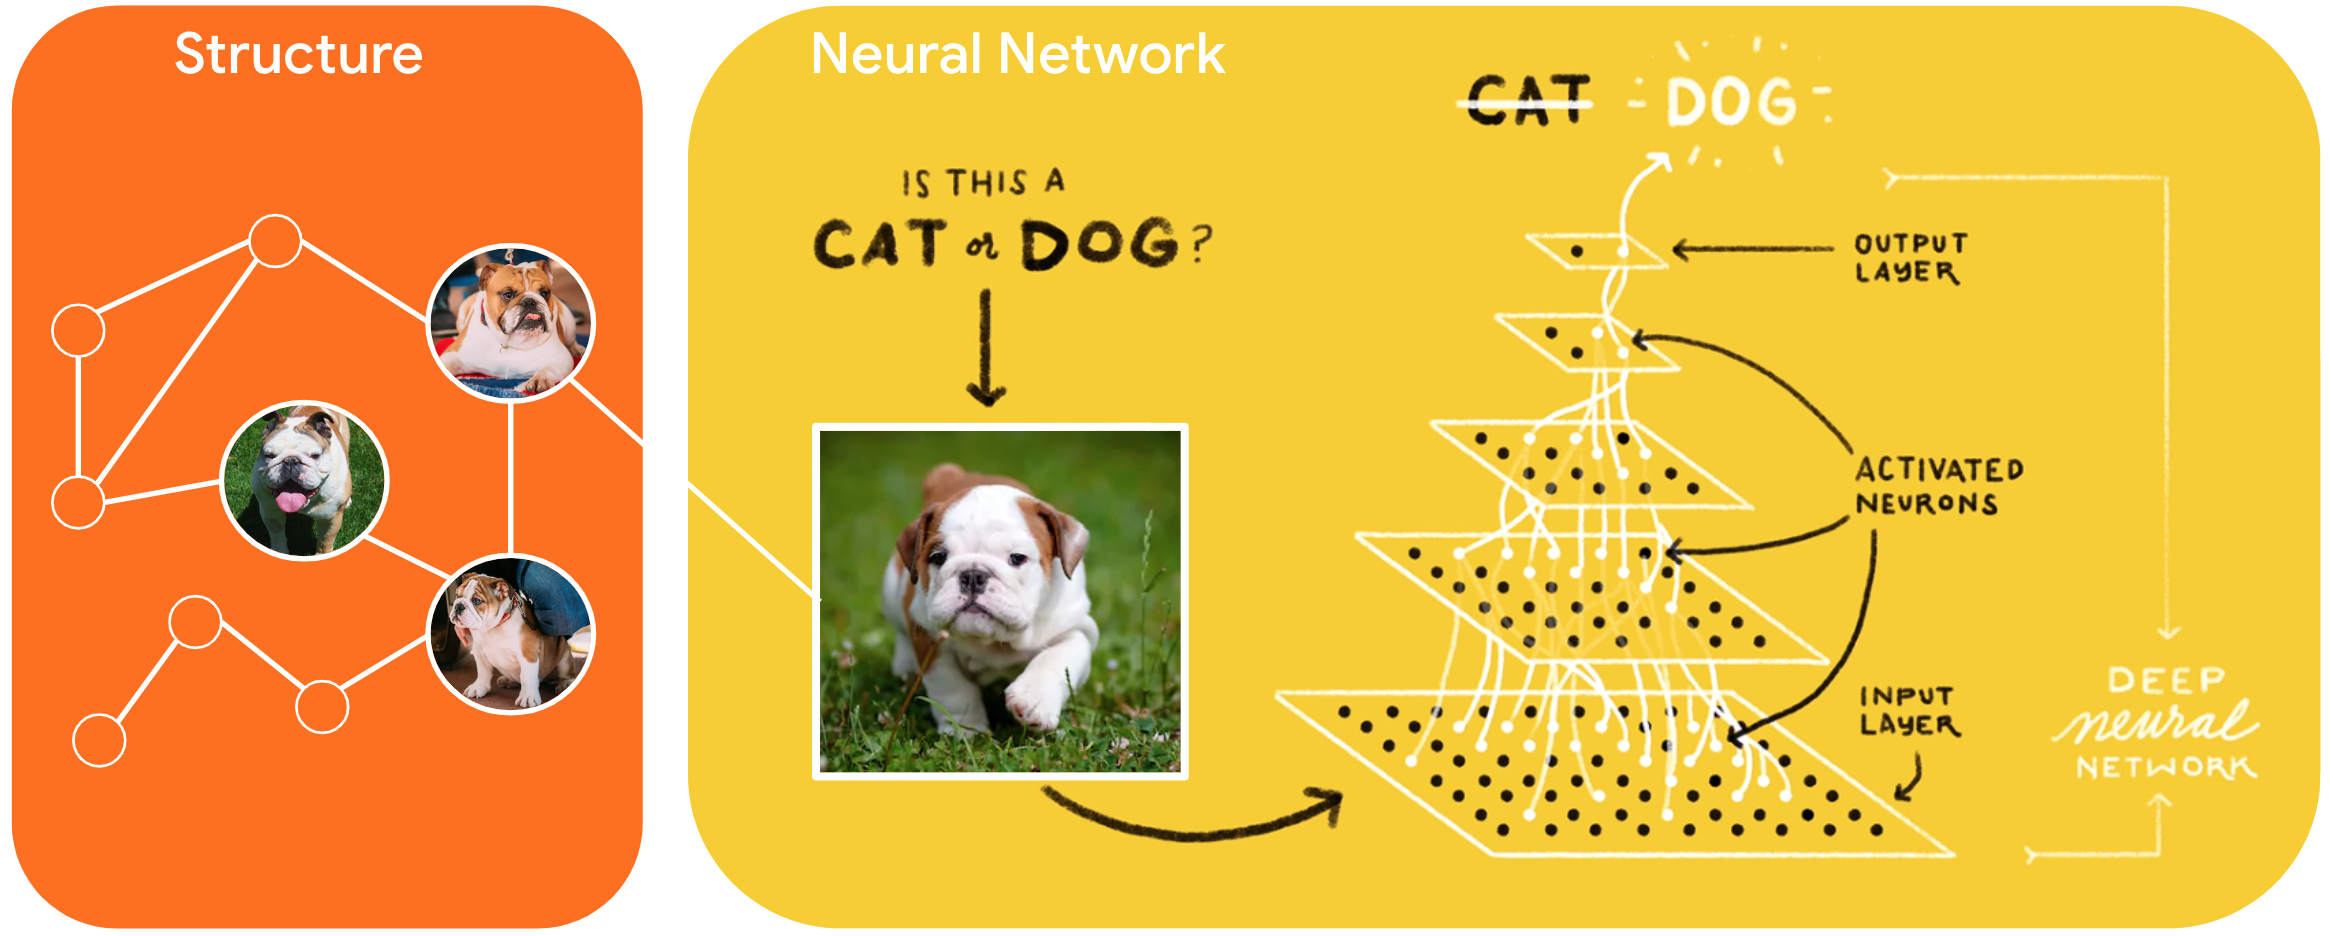
\includegraphics[width=0.8\linewidth]{Image/nsl_overview.png}
    \caption{Training with natural graphs}
    \label{Hình 1.3: Training with natural graphs}
    \cite*{WEBSITE:4}
\end{figure}

Về cơ bản, đồ thị tự nhiên là một tập hợp các điểm dữ liệu có mối quan hệ mật thiết với nhau, bản chất của mối quan hệ này có thể thay đổi dựa trên bối cảnh.
Mạng xã hội và Web là những ví dụ kinh điển mà chúng ta tương tác hàng ngày, ngoài những ví dụ này, chúng còn thường xuất hiện trong dữ liệu thường được sử dụng
cho nhiều nhiệm vụ học máy. Ví dụ khi ta cố gắng nắm bắt hành vi của người dùng dựa trên tương tác của họ với dữ liệu, thì việc lập mô hình dữ liệu dưới dạng biểu đồ 
có thể hợp lý. Đối với xử lý ngôn ngữ tự nhiên, chúng ta có thể định nghĩa một biểu đồ văn bản trong đó các nút biểu thị các thực thể và các cạnh biểu thị mối quan hệ 
giữa các cặp thực thể.

Xem xét bài toán phân loại tài liệu. Ví dụ như những kỹ sư AI thường chỉ quan tâm đến các bài viết về học máy trên một chủ đề cụ thể như thị giác máy tính hoặc xử lý ngôn ngữ
tự nhiên hoặc học tăng cường. Và thông thường, chúng ta có rất nhiều tài liệu hoặc giấy tờ như thế để phân loại, nhưng rất ít trong số chúng có nhãn. Vì vậy cần phải làm cho 
dữ liệu được thiết lập thành một biểu đồ tự nhiên, điều này nghĩa là nếu một bài báo hoặc tài liệu được trích dẫn từ bài báo hoặc tài liệu khác thì chúng có thể có cùng nhãn.
Việc sử dụng các thông tin quan hệ như vậy từ biểu đồ trích dẫn tận dụng được cả các mẫu được gắn nhãn cũng như không được gẵn nhãn. Điều này có thể bù đắp cho việc thiếu nhãn 
trong dữ liệu đào tạo. Vì vậy, việc xây dựng các đồ thị tự nhiên là rất cần thiết để giúp đào tạo các mô hình học máy một cách hiệu quả hơn.

\textbf{Traning with synthesized graphs}

\begin{figure}[h!]
    \centering
    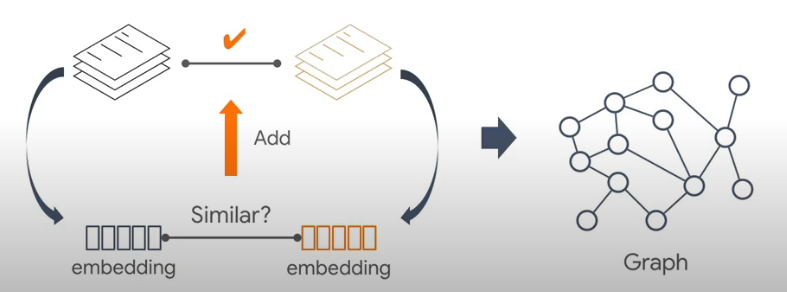
\includegraphics[width=0.8\linewidth]{Image/Graph2.png}
    \caption{Traning with synthesized graphs}
    \label{Hình 1.3: Traning with synthesized graphs}
    \cite*{WEBSITE:4}
\end{figure}

Mặc dù đồ thị tự nhiên là phổ biến, tuy nhiên có nhiều bài toán học máy với dữ liệu đầu vào không tạo thành đồ thị tự nhiên.
Ví dụ như phân loại văn bản đơn giản hoặc phân loại hình ảnh thì dữ liệu đầu vào chỉ chứa hình ảnh hoặc văn bản thô, do đó ta không thể 
tạo ra biểu đồ tự nhiên. Vì vậy Training with synthesized graphs được sử dụng để giải quyết vấn đề này. Với ý tưởng chính là xây dựng hoặc tổng hợp một biểu đồ từ dữ liệu đầu vào.
Trong Training with synthesized graphs chúng ta vẫn sự dụng sự giống nhau giữa các dữ liệu để xây dựng biểu đồ. Để xác định số liệu tương tự, thì cần phải chuyển đổi các văn bản thô hoặc
hình ảnh thành các thành phần nhúng tương ứng hoặc các biểu diễn dày đặc. Khi chuyển đổi dữ liệu thành các thành phần nhúng tương ứng, thì ta có thể sử dụng các mô hình đào tạo trước đó hoặc 
một số hàm chẳng hạn như cos để so sánh mức độ tương ứng giữa của các cặp phần nhúng. Nếu điểm tương đồng lớn hơn một ngưỡng nhất định thì ta sẽ thêm vào một cạnh tương ứng vào biểu đồ kết quả.
Việc lặp lại quy trình này sẽ bao phủ toàn bộ tập dữ liệu và sẽ tạo ra một biểu đồ. Và khi ta có biểu đồ thì việc sử dụng phương pháp học có cấu trúc trung tính rất đơn giản.


\subsection{Adversarial Learning}

\subsubsection*{Adversarial examples}

Adversarial example là các mẫu được tạo ra với những thao tác tinh vi bằng cách thêm vào các nhiễu đối nghịch nhỏ mà mắt người không thể nào nhìn thấy được đã biến nó thành một hình ảnh hoàn toàn khác dưới con mắt kỹ thuật số của thuật 
toán machine learning.

Một số mô hình học máy bao gồm các mạng lưới thần kinh hiện đại nhất, dễ bị sai lệch trước những Adversarial examples. Những mô hình này cho ra kết quả sai các ví dụ chỉ khác một chút so với các ví dụ được phân loại chính xác từ trong tập 
dữ liệu. Ví dụ như khi chúng ta đưa ra đặc điểm của một con gấu trúc thì chúng ta sẽ tìm những đặc trưng của nó như mắt đen, đầu tròn, thân trắng... Nhưng đối với một mạng neural nhân tạo, miễn là khi dữ liệu được đưa vào chạy qua các layer 
đưa ra kết quả trả lời đúng thì nó sẽ tin hình ảnh của dữ liệu đó là con gấu trúc.

\begin{figure}[h!]
    \centering
    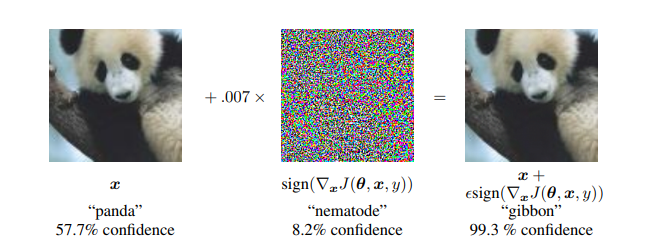
\includegraphics[width=0.8\linewidth]{Image/ADV.png}
    \caption{Adversarial examples}
    \label{Hình 1.4: Adversarial examples}
    \cite*{Reference7}
\end{figure}

Từ hình 2.4 ta thấy, khi thêm vào 1 vector tín hiệu nhiễu rất rất bé mà mắt người không thể phân biệt được sự khác nhau giữa hai hình ảnh của con gấu trúc thì nó đã đánh lừa được mạng neural và khiến nó phán đoán sai và nó tin chắc rằng
thứ mà nó đang nhìn thấy là con vượn (99.3\%). Điều này cho thấy khi các tập dữ liệu không tốt(có nhiễu) thì có thể khiến mạng neural đưa ra phán đoán sai.
 Để giải quyết vấn đề này, Adversarial training được đề xuất để dạy các mạng neural không bị đánh lừa và phân loại sai. 

\cite*{Reference6}
\textbf{Adversarial training}

Khái niệm về Adversarial training liên quan đến việc đào tạo bộ phân loại để khái quát hóa
Adversarial examples cũng như mẫu sạch. Trong lược đồ đào tạo thông thường, được hiển thị trong Hình 2.5, dữ liệu đào tạo chuyển tiếp
thông qua mô hình và tổn thất dự đoán được lan truyền ngược để cải thiện phân loại
kết quả. Kết quả là, mô hình sẽ khái quát hóa việc phân phối dữ liệu huấn luyện để
đưa ra một dự đoán chính xác về nhãn. 

Để đào tạo mô hình tránh bị nhầm lẫn khi tập dữ liệu có nhiễu thì ta sẽ tạo ra các dữ liệu có nhiễu nhỏ từ tập dữ liệu đào tạo
sau đó thêm các cạnh để kết nối dữ liệu vừa tạo ra với các mẫu của nó để xây dựng một cấu trúc linh hoạt sau đó, cấu trúc này có thể được sử dụng trong khung học tập
của cấu trúc thần kinh. Trong khung học cấu trúc thần kinh, mạng thần kinh cố gắng học cách duy trì cấu trúc bằng cách giữ sự giống nhau giữa một mẫu và hàng xóm của nó.
 Vì vậy về cơ bản việc sử dụng tập dữ liệu sạch và dữ liệu đối nghịch của nó sẽ nói với mạng thần kinh rằng mẫu và mẫu đối nghịch của nó thực sự giống nhau. Vì vậy, hãy giữ sự 
 giống nhau giữa chúng và đừng bị nhầm lẫn bởi các nhiễu.

\begin{figure}[h!]
    \centering
    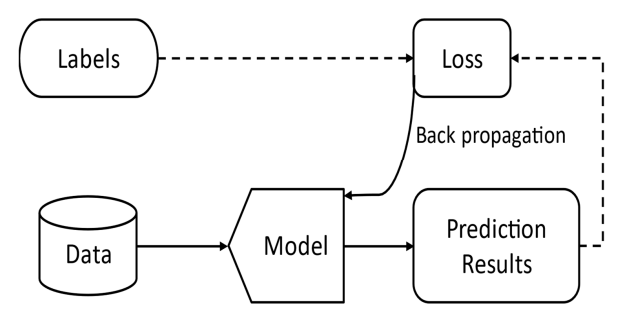
\includegraphics[width=0.72\linewidth]{Image/ADVT1.png}
    \caption{Basic training}
    \label{Hình 2.5: Adversarial training}
    \cite*{Reference8}
\end{figure}

Adversarial training mở rộng các phương pháp đào tạo thông thường bằng cách bổ sung thêm
bước vào quy trình đào tạo, như được minh họa trong Hình 2.6. Bằng cách này, mô hình có thể
khái quát hóa cả dữ liệu sạch và dữ liệu đối nghịch được tạo ra bởi các phương thức
được sử dụng trong Adversarial training để chống lại sự đánh lừa của mẫu đối nghịch.

\begin{figure}[h!]
    \centering
    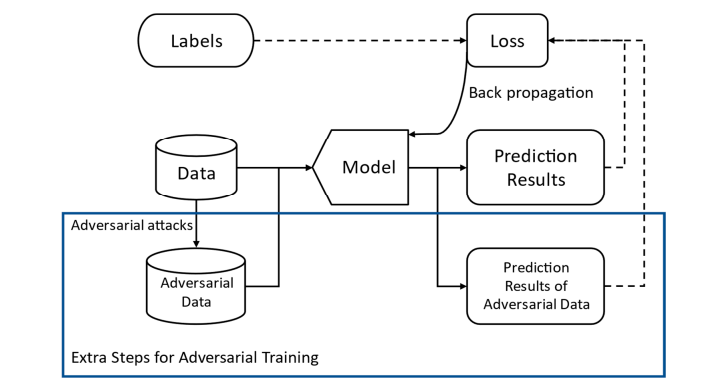
\includegraphics[width=0.72\linewidth]{Image/ADVT2.png}
    \caption{Adversarial training}
    \label{Hình 2.6: Adversarial training}
    \cite*{Reference8}
\end{figure}

Trong thư viện TensorFlow có sẵn các hàm chức năng để tạo ra các mẫu đối ngịch. 
Tương tự thì Keras API cũng có thể sử dụng để cho phép đào tạo từ đầu đến cuối
một cách dễ dàng với Adversarial training như: AdversarialRegularization, AdvNeighborConfig, AdvRegConfig...

\section{Adversarial Regularization for Image Classification}
\subsection{Chuẩn bị dữ liệu}

Ở phần trước chúng ta đã đi qua tổng quan về TensorFLow và Neural Structured Learning. Tuy nhiên để làm rõ hơn về hiệu quả của Neural
Structured Learning, chúng ta cần thực nghiệm trên một bài toán thực tế. Vì vậy ta sẽ ứng dụng Neural Structured Learning và chính xác hơn là Adversarial 
Regularization for Image Classification.
\begin{figure}[h!]
    \centering
    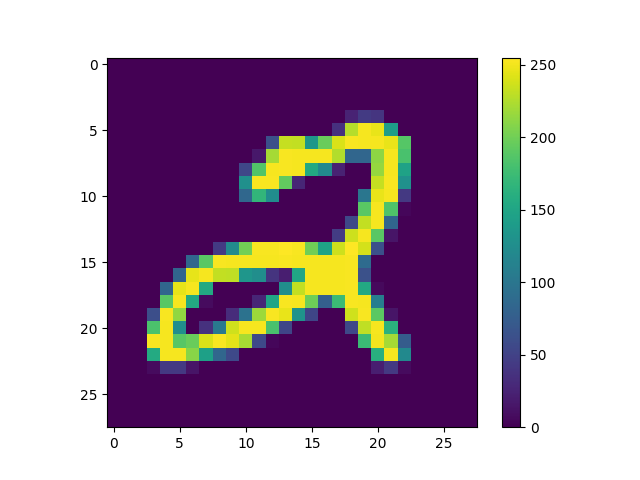
\includegraphics[width=0.6\linewidth]{Image/data.png}
    \caption{Ảnh chữ số viết tay được lấy từ tập dữ liệu MNIST}
    \label{Hình 2.7: GẢnh chữ số viết tay được lấy từ tập dữ liệu MNIST}
\end{figure}


Dựa trên tập dữ liệu có sẵn của thư viện TensorFlow MNIST, chúng ta sẽ thực hiện một bài toán phân loại ảnh chữ số viết tay. Tập dữ liệu bao gồm 70.000 ảnh
chữ số viết tay được chia thành 60.000 ảnh để huấn luyện và 10.000 ảnh để kiểm tra. Mỗi ảnh có kích thước 28x28 pixel và được biểu diễn dưới dạng một mảng
2 chiều 28x28. Mỗi phần tử trong mảng này là một giá trị từ 0 đến 255 biểu diễn độ sáng của một pixel. Để thuận tiện cho việc huấn luyện, chúng ta sẽ chuyển đổi
mỗi ảnh thành một mảng 1 chiều 784 phần tử. Để đơn giản hơn, chúng ta sẽ chia tập dữ liệu thành 2 tập huấn luyện và kiểm tra. Tập huấn luyện sẽ bao gồm 60.000 ảnh 
và tập kiểm tra sẽ bao gồm 10.000 ảnh. Mỗi ảnh sẽ được gán nhãn là một số từ 0 đến 9 tương ứng với chữ số viết tay. 

\subsection{Mô hình}
Chúng ta có thể sử dụng các mạng neural thông thường để xây dựng mô hình phán đoán chữ số. Ý tưởng là sử dụng một vài mạng neural để tính toán các trọng số
của mô hình. 
\begin{equation}
    \begin{aligned}  
      w_1X_1 + w_2X_2 + ... + w_nX_n = y\\
    \end{aligned}
\end{equation}

trong đó:
\begin{itemize}
    \item $w_1, w_2, ..., w_n$ là các trọng số của mô hình.
    \item $X_1, X_2, ..., X_n$ là giá trị của các pixel.
    \item $y$ là giá trị dự đoán của mô hình.
\end{itemize}


Mô hình sẽ tìm kiếm các trọng số phù hợp để đưa ra được đầu ra y chính xác đối với các hình ảnh đầu vào.
Tuy nhiên nếu thưc hiện như vậy, chúng ta sẽ không thể đạt được kết quả tốt. Vì vậy chúng ta cần phải sử dụng một số kỹ thuật để cải thiện độ chính xác của mô hình.
Bằng cách thêm các convolutional layer và pooling layer vào mô hình, chúng ta sẽ có thể giảm số lượng tham số của mô hình và cải thiện độ chính xác của mô hình.



Chúng ta sẽ thực hiện xây dựng và đào tạo một mạng neural đơn giản và một mạng neural sử dụng Adversarial Regularization. Sau đó chúng ta sẽ so sánh kết quả 
dự đoán của 2 mạng neural này để thấy được hiệu quả của Neural Structured Learning. Sau khi đào tạo và dự đoán thử trên tập dữ liệu có sẵn của TensorFlow, thì
ta sẽ thử viết tay một vài chữ số và để cho mạng neural dự đoán xem nó có thể dự đoán chính xác không.

Với những thư viện đồ sộ và khả năng làm việc với các ma trận tốt, Python là ngôn ngữ được lựa chọn để thực hiện ý tưởng trên. Cùng với đó là các thư viện như numpy, matplotlib và
đặc biệt là TensorFlow với API keras và Neural structed learning.



 
% Template cho một chương

\chapter{Adversarial regularization for image classification} % Tên của chương

\label{Chapter2} % Thay X bằng số chương tương ứng; để trích dẫn chương này ở chỗ nào đó trong bài, hãy sử dụng lệnh \ref{ChapterX} 

%----------------------------------------------------------------------------------------
%	MỤC 1
%----------------------------------------------------------------------------------------

\section{Đặt vấn đề}

Ở chương một chúng ta đã đi qua tổng quan về TensorFLow và Neural Structured Learning. Tuy nhiên để làm rõ hơn về hiệu quả của Neural
Structured Learning, chúng ta cần thực nghiệm trên một bài toán thực tế. Vì vậy ta sẽ ứng dụng Neural Structured Learning và chính xác hơn là Adversarial 
Regularization for Image Classification.

Dựa trên tập dữ liệu có sẵn của thư viện TensorFlow MNIST, chúng ta sẽ thực hiện một bài toán phân loại ảnh chữ số viết tay. Tập dữ liệu bao gồm 70.000 ảnh
chữ số viết tay được chia thành 60.000 ảnh để huấn luyện và 10.000 ảnh để kiểm tra. Mỗi ảnh có kích thước 28x28 pixel và được biểu diễn dưới dạng một mảng
2 chiều 28x28. Mỗi phần tử trong mảng này là một giá trị từ 0 đến 255 biểu diễn độ sáng của một pixel. Để thuận tiện cho việc huấn luyện, chúng ta sẽ chuyển đổi
mỗi ảnh thành một mảng 1 chiều 784 phần tử. Để đơn giản hơn, chúng ta sẽ chia tập dữ liệu thành 2 tập huấn luyện và kiểm tra. Tập huấn luyện sẽ bao gồm 60.000 ảnh 
và tập kiểm tra sẽ bao gồm 10.000 ảnh. Mỗi ảnh sẽ được gán nhãn là một số từ 0 đến 9 tương ứng với chữ số viết tay. 

\begin{figure}[h!]
    \centering
    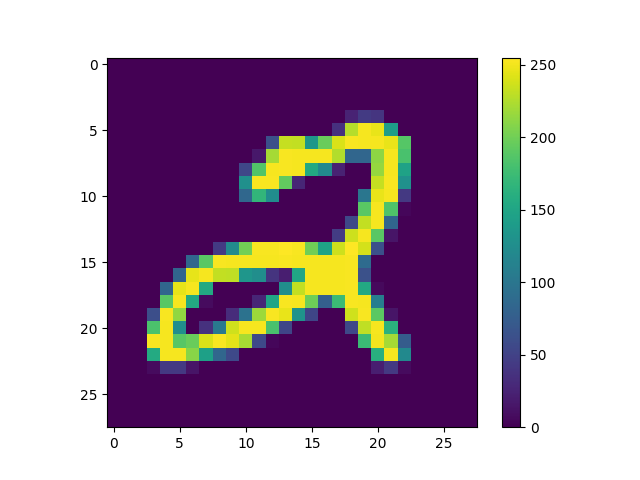
\includegraphics[width=0.6\linewidth]{Image/data.png}
    \caption{Ảnh chữ số viết tay được lấy từ tập dữ liệu MNIST}
    \label{Hình 2.1: GẢnh chữ số viết tay được lấy từ tập dữ liệu MNIST}
\end{figure}


Chúng ta sẽ thực hiện xây dựng và đào tạo một mạng neural đơn giản và một mạng neural sử dụng Adversarial Regularization. Sau đó chúng ta sẽ so sánh kết quả 
dự đoán của 2 mạng neural này để thấy được hiệu quả của Neural Structured Learning. Sau khi đào tạo và dự đoán thử trên tập dữ liệu có sẵn của TensorFlow, thì
ta sẽ thử viết tay một vài chữ số và để cho mạng neural dự đoán xem nó có thể dự đoán chính xác không.

Với những thư viện đồ sộ và khả năng làm việc với các ma trận tốt, Python là ngôn ngữ được lựa chọn để thực hiện ý tưởng trên. Cùng với đó là các thư viện như numpy, matplotlib và
đặc biệt là TensorFlow với API keras và Neural structed learning.





%----------------------------------------------------------------------------------------
%	MỤC 2
%----------------------------------------------------------------------------------------

\section{Thực nghiệm}

\subsection{Cài đặt môi trường}

Bước đầu tiên cần cài đặt biến môi trường và các thư viện cần thiết. Cài đặt phiên bản python3 và editor hoặc IDE để viết mã như Pycharm hoặc VScode.
Sau đó, trên command line chạy dòng lệnh 'pip install -r Setup.txt' để tiến hành cài đặt các thư viện cần thiết. File "Setup.txt" là file chứa các thư viện 
cần cài đặt.

\subsection{Viết mã}
\textbf{Import thư viện}
% insert code python
\begin{lstlisting}[language=Python]
    import tensorflow as tf
    import numpy as np
    import neural_structured_learning as nsl
    import matplotlib.pyplot as plt
    import tensorflow_datasets as tfds
\end{lstlisting}

\textbf{Khai báo các tham số}
% insert code python
\begin{lstlisting}[language=Python]
    input_shape = [28, 28, 1]
    num_classes = 10
    conv_filters = [32, 64, 64]
    kernel_size = (3, 3)
    pool_size = (2, 2)
    num_fc_units = [64]
    batch_size = 32
    epochs = 5
    adv_multiplier = 0.2
    adv_step_size = 0.2
    adv_grad_norm = 'infinity'
\end{lstlisting}

Khai báo các tham số cần thiết cho việc xây dựng mạng neural và đào tạo. Các tham số được khai báo như sau:

Đầu vào và đầu ra:
\begin{itemize}
    %highlight Item name
    \item \textbf{input\_shape}: Hình dạng của tensor đầu vào. Mỗi hình ảnh có kích thước 28x28pixel và có 1 kênh màu.
    \item \textbf{num\_classes}: Số lượng lớp đầu ra. Trong bài toán này là 10 lớp từ 0 đến 9.
\end{itemize}

Các tham số để xây dựng mô hình mạng neural:
\begin{itemize}
    %highlight Item name
    \item \textbf{conv\_filters}: Số lượng lọc cho mỗi lớp tích chập. Mỗi lớp tích chập có số bộ lọc bao gồm 32,64,64.
    \item \textbf{kernel\_size}: Kích thước của kernel tích chập 2D. Mỗi kernel có kích thước 3x3.
    \item \textbf{pool\_size}: Các yếu tố để thu nhỏ hình ảnh trong mỗi lớp tổng tối đa. Mỗi pooling có kích thước 2x2.
    \item \textbf{num\_fc\_units}: Số lượng đơn vị ẩn của mỗi lớp fully connected. Mỗi lớp fully connected có 64 đơn vị ẩn. Nghĩa là chiều rộng của mỗi lớp được kết nối đầy đủ.
\end{itemize}

Các tham số để đào tạo mô hình:
\begin{itemize}
    \item \textbf{batch\_size}: Kích thước batch. Mỗi batch có 32 hình ảnh. Là số lượng bức ảnh được đưa vào mạng neural mỗi lần.
    \item \textbf{epochs}: Số lần huấn luyện. Mỗi lần sẽ duyệt qua tất cả các hình ảnh trong tập dữ liệu.
    \item \textbf{adv\_multiplier}: Trọng số tổn thất do nhiễu loạn đối nghịch gây ra trong mục tiêu huấn luyện, so với tổn thất của mô hình gốc(tổn thất được gắn nhãn).
    \item \textbf{adv\_step\_size}: Độ lớn của nhiễu loạn đối nghịch.
    \item \textbf{adv\_grad\_norm}: Định mức để đo mức độ nhiễu loạn của đối nghịch. %Có 3 giá trị là 'infinity', 'l2', 'l1'.
\end{itemize}

\textbf{Tải dữ liệu MNIST}
% insert code python
\begin{lstlisting}[language=Python]
    data_train, data_test = tfds.load('mnist', split=['train', 'test'])
\end{lstlisting}

Bộ dữ liệu MNIST chứa hình ảnh thang độ xám của các chữ số viết tay từ 0 dến 9. Mỗi hình ảnh hình ảnh hiển thị một chữ số ở độ phân giải thấp 28x28 pixel.
Nhiệm vụ liên quan là phân loại hình ảnh thành 10 loại, mỗi loại tương ứng với một chữ số từ 0 đến 9.

Bộ dữ liệu đã có sẵn trong thư viện TensorFlow Datasets (TFDS) và có thể được tải xuống và xây dựng tệp tf.data.Dataset.
Tập dữ liệu đã tải bao gồm hai tập con :
\begin{itemize}
    \item \textbf{train}: Tập dữ liệu huấn luyện với 60000 ảnh.
    \item \textbf{test}: Tập dữ liệu kiểm tra với 10000 ảnh.
\end{itemize}

Các dữ liệu trong cả hai tập đều được lưu trữ dưới dạng dictionary với hai khóa:
\begin{itemize}
    \item \textbf{image}: Là các mảng pixel 28x28 chứa các giá trị từ 0 đến 255.
    \item \textbf{label}: Nhãn thật của hình ảnh, là một số nguyên từ 0 đến 9.
\end{itemize}

\begin{lstlisting}[language=Python]
    def normalize(features):
        features['image'] = tf.cast(features['image'], dtype=tf.float32) / 255.0
        return features

    def convert_to_tuples(features):
        return features['image'], features['label']

    def convert_to_dictionaries(image, label):
        return {'image': image, 'label': label}

    data_train = data_train.map(normalize).shuffle(10000).batch(batch_size).map(convert_to_tuples)
    data_test = data_test.map(normalize).batch(batch_size).map(convert_to_tuples)

\end{lstlisting}

Để làm cho mô hình ổn định về số lượng, chúng ta chuẩn hóa các giá trị pixel từ [0,255] thành [0, 1] bằng cách ánh xạ tập dữ liệu qua hàm normalize(). Sau khi xáo 
trộn tập huấn luyện và chia theo nhóm, chúng ta chuyển đổi các ví dụ thành các bộ dữ liệu đặc trưng (image, label) để huấn luyện mô hình cơ sở. Chúng ta 
cũng cung cấp một hàm chức năng để chuyển đổi từ bộ sang từ điển để sử dụng sau này.

\textbf{Xây dựng và đào tạo mô hình cơ bản}

Mô hình cơ bản sẽ là một mạng thần kinh bao gồm 3 lớp tích chập, theo sau là 2 lớp được kết nối đầy đủ ( với các tham số như được định nghĩa trong phần khai báo tham số). 
Trong đó các lớp tích chập sẽ có hàm kích hoạt activation là 'relu' còn hai lớp theo sau thì một lớp có hàm kích hoạt là 'relu'và lớp output sẽ là 'softmax'. Lớp output sử dụng 
activation 'softmax' để đánh giá xác suất phân loại dữ liệu đầu vào và tính toán trọng số cho dữ liệu.
Chúng ta tạo hàm build\_model() để thuận tiện cho việc tái sử dụng khi khởi tạo mô hình khác. 
Ở đây chúng ta xác định nó bằng các hàm API của Keras. 

\begin{lstlisting}[language=Python]
    def build_model():
        inputs = tf.keras.Input(shape=input_shape, dtype=tf.float32, name='image')
        x = inputs
        for i, num_filters in enumerate(conv_filters):
            x = tf.keras.layers.Conv2D(num_filters, kernel_size, activation='relu')(x)
            if i < len(conv_filters) - 1:
                x = tf.keras.layers.MaxPooling2D(pool_size)(x)
        x = tf.keras.layers.Flatten()(x)
        for num_units in num_fc_units:
            x = tf.keras.layers.Dense(num_units, activation='relu')(x)
        outputs = tf.keras.layers.Dense(num_classes, activation='softmax')(x)
        return tf.keras.Model(inputs=inputs, outputs=outputs)

    model_base = build_model()
\end{lstlisting}

Sau khi xây dựng model thì chúng ta sẽ tiến hành đào tạo và đánh giá model. Với hàm tối ưu hóa 'Adam' như đã giới thiệu ở phần trước, hàm mất mát 'SparseCategoricalCrossentropy'
và đánh giá 'SparseCategoricalAccuracy'. Sau khi đào tạo xong chúng ta sẽ đánh giá model bằng hàm evaluate() và in ra độ chính xác của model.

\begin{lstlisting}[language=Python]
model_base.compile(
    optimizer=tf.keras.optimizers.Adam(),
    loss=tf.keras.losses.SparseCategoricalCrossentropy(),
    metrics=[tf.keras.metrics.SparseCategoricalAccuracy()])
model_base.summary()

model_base_history = model_base.fit(data_train, epochs=epochs)

results = model_base.evaluate(data_test)
named_results = dict(zip(model_base.metrics_names, results))
print('\naccuracy:', named_results['sparse_categorical_accuracy'])

\end{lstlisting}

\begin{figure}[ht]
\centering
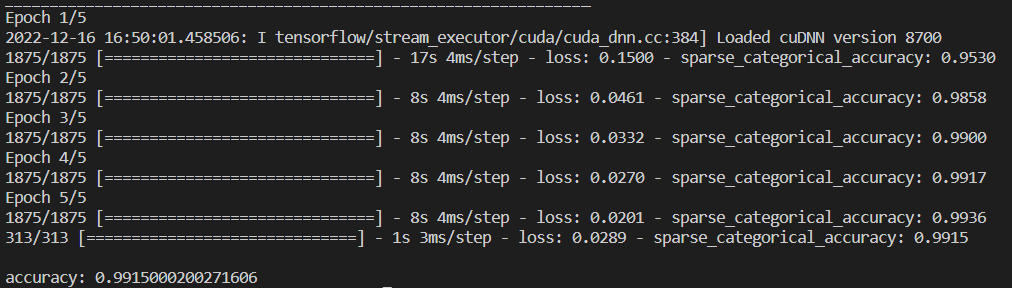
\includegraphics[width=\textwidth]{Image/base_acc.png}
\caption{Accuracy}
\label{fig2.2:Độ chính xác của mô hình cơ bản}
\end{figure}

Chúng ta có thể thấy rằng mô hình cơ bản đạt được độ chính xác lên đến 99,15\% trên bộ thử nghiệm. Từ đó cho thấy dữ liệu đào tạo và 
mô hình đào tạo là khá tốt. Tuy nhiên cần phải sử dụng các tập dữ liệu khác để đánh giá mô hình một cách chính xác hơn.

\textbf{Xây dựng và đào tạo mô hình Adversarial-regularized }

Chúng ta sẽ xây dựng mô hình mạng neural đối nghịch bằng cách kết hợp adversarial training vào mô hình keras và sử dụng khung Neural Structured Learning (NSL).
Mô hình cơ sở được bao bọc để tạo một mô hình mới \textbf{tf.Keras.Model}, có mục tiêu đào tạo bao gồm adversarial regularization.

Đầu tiên, chúng tôi tạo một đối tượng cấu hình với tất cả cáctham số có liên quan bằng cách sử dụng hàm chức năng \textbf{nsl.configs.make\_adv\_reg\_config} có sẵn trong thư viện NSL.

\begin{lstlisting}[language=Python]
    adv_config = nsl.configs.make_adv_reg_config(multiplier=adv_multiplier, 
        adv_step_size=adv_step_size, 
        adv_grad_norm=adv_grad_norm)
\end{lstlisting}

Ở đây chúng ta sẽ tạo một mô hình cơ bản mới \textbf{base\_adv\_model} để mô hình hiện tại (\textbf{model\_base}) dùng để so sánh sau này.

Bây giờ chúng ta có thể bọc một mô hình cơ sở bằng \textbf{AdversarialRegularization} bằng cách sử dụng hàm chức năng
có sẵn \textbf{nsl.keras.AdversarialRegularization}.

\begin{lstlisting}[language=Python]
    base_adv_model = build_model()
    model_adv = nsl.keras.AdversarialRegularization(
        base_adv_model,
        label_keys=['label'],
        adv_config=adv_config)

    data_train_adv = data_train.map(convert_to_dictionaries)
    data_test_adv = data_test.map(convert_to_dictionaries)
\end{lstlisting}

Trả về \textbf{adv\_model} là một đối tượng có kiểu \textbf{tf.keras.Model}, có mục tiêu đào tạo bao gồm phần regularization và mất mát của adveresarial. Để tính toán tổn thất đó, mô hình phải có quyền truy cập 
vào thông tin nhãn (feature label), ngoài đầu vào thông thường (feature image). Vì lý do này, chúng ta sẽ chuyển đổi các mẫu trong tập dữ liệu trở lại kiểu dictionary. Và chúng ta cho mô 
hình biết tính năng nào chứa thông tin nhãn thông qua tham số \textbf{label\_keys}.

Tiếp theo, chúng ta sẽ biên dịch, đào tạo và đánh giá mô hình chính quy hóa đối thủ. Với các hàm tối ưu, mất mát, và đánh giá độ chính xác tương tự như khi đào tạo mô hình cơ bản.
Có thể có các cảnh báo như "Output missing from loss dictionary", điều này không sao cả vì \textbf{adv\_model} không dựa vào triển khai cơ sở để tính tổng tổn thất.



\begin{lstlisting}[language=Python]
    model_adv.compile(
        optimizer=tf.keras.optimizers.Adam(),
        loss=tf.keras.losses.SparseCategoricalCrossentropy(),
        metrics=[tf.keras.metrics.SparseCategoricalAccuracy()])

    model_adv_history = model_adv.fit(data_train_adv, epochs=epochs)
    
    adv_results = model_adv.evaluate(data_test_adv)
    named_adv_results = dict(zip(model_adv.metrics_names, adv_results))
    print('\naccuracy:', named_adv_results['sparse_categorical_accuracy'])

\end{lstlisting}

\begin{figure}[h!]
    \centering
    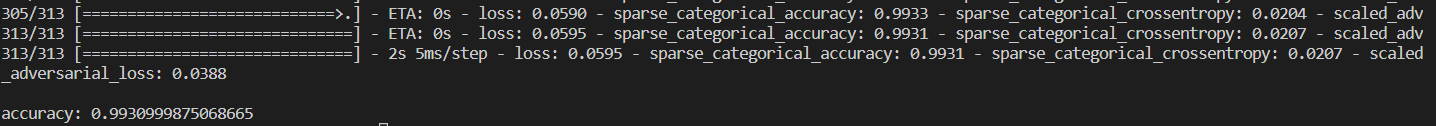
\includegraphics[width=\textwidth]{Image/adv_acc.png}
    \caption{Độ chính xác của mô hình Adversarial-regularized.}
    \label{fig 2.3:Độ chính xác của mô hình Adversarial-regularized}
\end{figure}

Chúng ta có thể thấy rằng mô hình Adversarial-regularized cũng hoạt động rất tốt (độ chính xác 99,31\%) trên tập thử nghiệm. Tuy độ chính xác có nhỉnh hơn một xíu so với mô hình cơ bản
nhưng không quá nhiều.

Chúng ta sẽ đưa ra đồ thị sự thay đổi của độ chính xác qua mỗi lần học tập trên tập dữ liệu thử nghiệm của cả hai mô hình để dễ dàng quan sát hơn.
\begin{lstlisting}[language=Python]
    plt.plot(model_base_history.history['sparse_categorical_accuracy'])
    plt.plot(model_adv_history.history['sparse_categorical_accuracy'])
    plt.title('model accuracy')
    plt.ylabel('accuracy')
    plt.xlabel('epoch')
    plt.legend(['base', 'adversarial'], loc='upper left')
    plt.show()
\end{lstlisting}

\begin{figure}[h!]
    \centering
    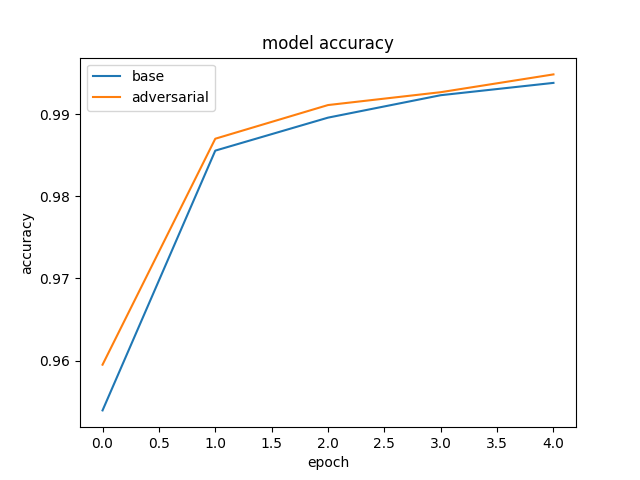
\includegraphics[width=0.7\textwidth]{Image/plt.png}
    \caption{Đồ thị độ chính xác của hai mô hình qua từng lần học.}
    \label{fig 2.4:Đồ thị độ chính xác của hai mô hình qua từng lần học.}
    
\end{figure}

Từ đồ thị, ta thấy đường cong độ chính xác của mô hình Adversarial-regularized và mô hình cơ bản có xu hướng tương tự nhau. Mô hình adversarial-regularized có nhỉnh hơn một chút nhưng chênh lệch là không quá nhiều. 
Điều này là do cả hai mô hình đều sử dụng các hàm tối ưu, mất mát và đánh giá tương tự nhau.

\textbf{So sánh độ chính xác của hai mô hình dưới các mẫu nhiễu loạn đối nghịch}

Bây giờ chúng ta so sánh mô hình cơ sở và mô hình Adversarial-regularized về khả năng phán đoán chính xác dưới sự nhiễu loạn của các mẫu đối nghịch.
Chúng ta sẽ sử dụng hàm chức năng \textbf{AdversarialRegularization.perturb\_on\_batch()} để tạo các mẫu nhiễu loạn đối nghịch. Để có thể sánh được độ chính xác của hai mô hình,
ta sẽ phải bọc mô hình cơ bản bằng \textbf{AdversarialRegularization}. Các biến mà mô hình cơ bản đã học trước đó sẽ không bị thay đổi miễn là chúng ta không gọi hàm đào tạo \textbf{fit()}.

\begin{lstlisting}[language = Python]
    ref_model = nsl.keras.AdversarialRegularization(
        model_base,
        label_keys=['label'],
        adv_config=adv_config)


    ref_model.compile(
        optimizer=tf.keras.optimizers.Adam(),
        loss=tf.keras.losses.SparseCategoricalCrossentropy(),
        metrics=[tf.keras.metrics.SparseCategoricalAccuracy()])
\end{lstlisting}

Tiếp theo chúng ta sẽ đánh giá và so sánh khả năng phán đoán của hai mô hình trên các mẫu đối nghịch.
Ở đây chúng ta lấy \textbf{adv\_model.base\_model} để có cùng định dạng đầu vào (không yêu cầu thông tin nhãn) làm mô hình cơ sở. Các biến đã học trong \textbf{adv\_model.base\_model} giống như các biến 
trong \textbf{adv\_model}.

\begin{lstlisting}[language = Python]
    models_to_evaluate = {
        'base': model_base,
        'adversarial': model_adv.base_model,
    }

    metrics = {
        name: tf.keras.metrics.SparseCategoricalAccuracy()
        for name in models_to_evaluate.keys()
    }    
\end{lstlisting}

Tiếp theo chúng ta sẽ tạo các ví dụ nhiễu loạn và đánh giá các mô hình với chúng. Chúng ta lưu các hình ảnh, nhãn và dự đoán bị nhiễu vào 3 mảng perturbed\_imgs,labels,predictions để trực 
quan hóa trong phần sau để có cách nhìn rõ hơn về khả năng phán đoán của hai mô hình. Các mẫu nhiễu loạn được tạo ra từ tập dữ liệu test và
được chuẩn hóa để chúng có cung kích thước với các mẫu thông thường bằng hàm chức năng \textbf{tf.clip\_by\_value}.


\begin{lstlisting}[language = Python]
    perturbed_imgs,labels,predictions = [],[],[]

    for batch in data_test_adv:
        perturbed_batch = ref_model.perturb_on_batch(batch)
        perturbed_batch['image'] = tf.clip_by_value(perturbed_batch['image'], 0, 1)

        y_true = perturbed_batch.pop('label')
        perturbed_imgs.append(perturbed_batch['image'].numpy())
        labels.append(y_true.numpy())
        predictions.append({})

        for name, model in models_to_evaluate.items():
            y_pred = model(perturbed_batch)
            metrics[name].update_state(y_true, y_pred)
            predictions[-1][name] = tf.argmax(y_pred, axis=-1).numpy()

    for name, metric in metrics.items():
        print(f'{name} accuracy: {metric.result().numpy()}')

\end{lstlisting}

\begin{figure}[h!]
    \centering
    
\includegraphics[width=\textwidth]{Image/acc.png}
    \caption{Độ chính xác của hai mô hình trên mẫu nhiễu loạn đối nghịch.}
    \label{fig 2.5:Độ chính xác của hai mô hình trên mẫu nhiễu loạn đối nghịch.}
    
\end{figure}

Từ hình 2.5 Chúng ta có thể thấy rằng độ chính xác của mô hình cơ bản giảm đáng kể (từ 99,15\% xuống còn khoảng 57,7\%) khi đầu vào bị nhiễu. Mặt khác, 
độ chính xác của mô hình Adversarial-regularized chỉ giảm một chút (từ 99,31\% xuống 96,2\%). Điều này chứng tỏ tính hiệu quả của việc học đối thủ trong 
việc cải thiện độ chính của mô hình và khả năng hoạt động tốt của mô hình trên những tập dữ liệu nhiều nhiễu.

\textbf{Trực quan hóa các mẫu nhiễu loạn đối nghịch}

Chúng ta sẽ chọn ra một batch ngẫu nhiên trong mảng perturbed\_imgs đã lưu ở trên để trực quan hóa, ở đây batch được chọn là batch thứ 5.
Sử dụng thư viện \textbf{matplotlib} để hiển thị các hình ảnh và hiển thị các dự đoán của hai mô hình và kiểm tra xem mô hình đoán có đúng không so với
nhãn thật.


\begin{lstlisting}[language = Python]
    batch_index = 5

    batch_images = perturbed_imgs[batch_index]
    batch_labels = labels[batch_index]
    batch_predictions = predictions[batch_index]

    n_columns = 5
    n_rows = (batch_size + n_columns - 1) // n_columns

    print('acc in batch %d: ' % batch_index, end='')
    for name,pred in batch_predictions.items():
        print('%s model: %d / %d' % (name, np.sum(batch_labels == pred), batch_size))

    plt.figure(figsize=(n_columns * 2, n_rows * 2))
    for i,(img,y) in enumerate(zip(batch_images, batch_labels)):
        y_base = batch_predictions['base'][i]
        y_adv = batch_predictions['adversarial'][i]
        plt.subplot(n_rows, n_columns, i + 1)
        plt.title('true: %d, base: %d, adv: %d' % (y, y_base, y_adv))
        plt.imshow(img)
        plt.axis('off')

    plt.tight_layout()
    plt.show()

    
\end{lstlisting}

\begin{figure}[h!]
    \centering
    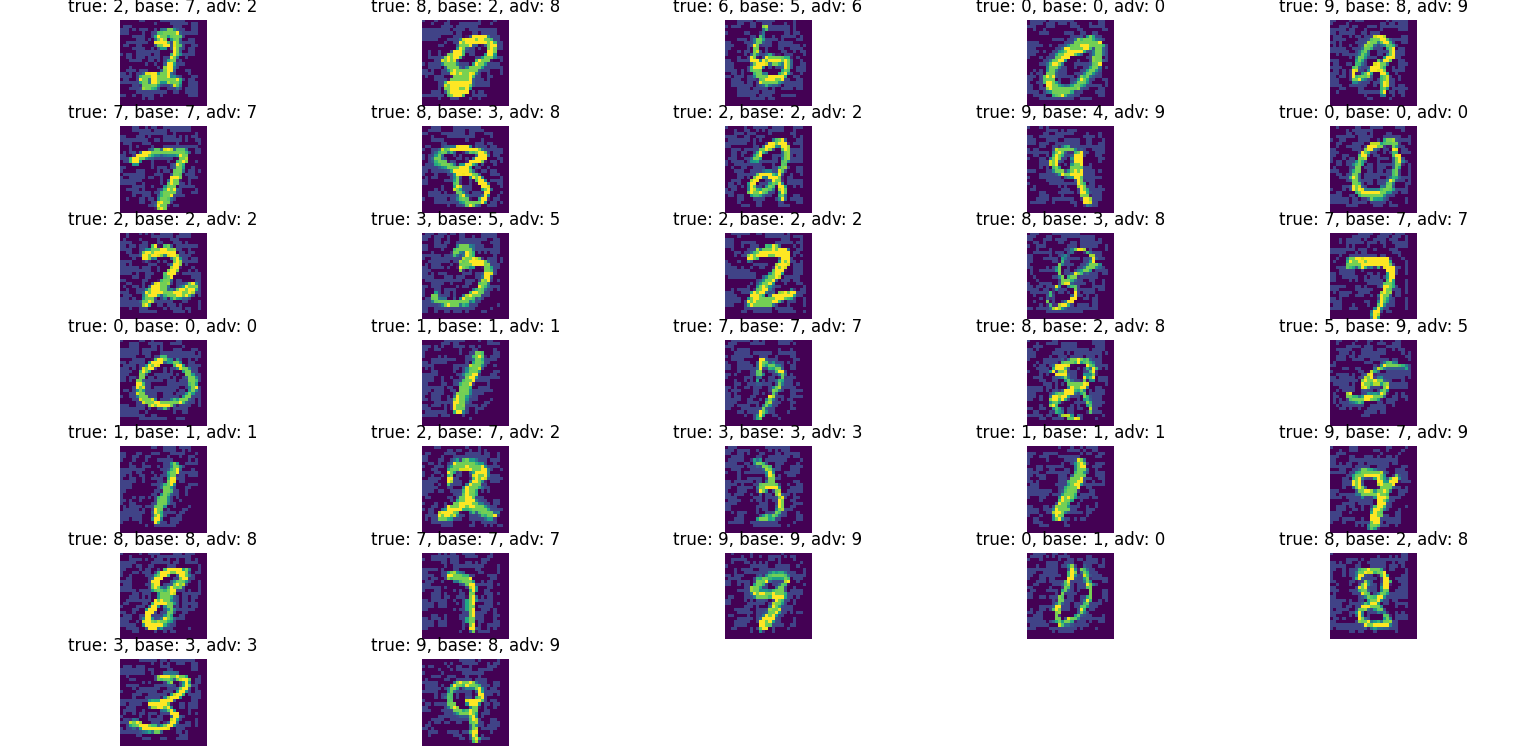
\includegraphics[width=\textwidth]{Image/result.png}
    \caption{Một số mẫu nhiễu loạn đối nghịch và các phán đoán của hai mô hình.}
    \label{fig 2.6:Một số mẫu nhiễu loạn đối nghịch và các phán đoán của hai mô hình.}
    
\end{figure}

\begin{figure}[h!]
    \centering
    
\includegraphics[width=\textwidth]{Image/acc_in_batch.png}
    \caption{Số dự đoán chính xác của hai mô hình trên mẫu nhiễu loạn đối nghịch trong batch 5.}
    \label{fig 2.7:Số dự đoán chính xác của hai mô hình trên mẫu nhiễu loạn đối nghịch trong batch 5.}
    
\end{figure}

Từ hình 2.6 ta thấy, các nhiễu loạn nhỏ được thêm vào những bức ảnh chữ số viết tay dưới mắt người vẫn có thể nhận biết được
tuy nhiên nó đã đánh lừa được mô hình cơ bản phán đoán sai.

Từ hình 2.7 ta thấy rằng, khả năng phán đoán của mô hình cơ bản(base model) khá thấp(21/32 mẫu). Trong khi đó
mô hình Adversarial-regularized phán đoán rất tốt (32/32 mẫu).


\textbf{Lưu mô hình vừa đào tạo}

Sau khi đào tạo chúng ta sẽ lưu lại các mô hình để thử cho các mô hình phán đoán một số hình ảnh viết tay không phải thuộc tập dữ
liệu của tensorflow\_datasets. Mô hình được lưu lại có thể dễ dàng mang ra sử dụng hoặc tiếp tục đào tạo tùy mục đích và no được lưu dưới định dạng '.h5' với sự hỗ trợ của
thư viện \textbf{h5py}. Lưu ý rằng, sau khi lưu mô hình thì các biến mà mô hình đã học tập được sẽ được giữ nguyên.

\begin{lstlisting}[language = Python]
    model_adv.save('Model/advs_model.h5')
    model_base.save('Model/base_model.h5')
\end{lstlisting}

\cite*{WEBSITE}

\subsection{Kiểm tra mô hình với một số ảnh viết tay}

Ở phần trước, chúng ta đã xây dựng, đào tạo và kiểm tra mô hình trên tập dữ liệu của tensorflow\_datasets. Tuy nhiên, chúng ta 
để biết được thực sự mô hình có hoạt động tốt với các bức ảnh ngẫu nhiên hay không, ta sẽ viết tay một số chữ số và cho mô hình dự đoán.

Ở phần này, chúng ta sẽ sử dụng thư viện xử lý ảnh OpenCV để đọc và tiền xử lý các bức ảnh chụp. Do đầu vào của mô hình là một bức ảnh 28x28
nên chúng ta cần phải resize ảnh về kích thước này. Sau đó, chúng ta cũng cần chuyển ảnh về dạng mảng numpy với giá trị trong khoảng 0-1 để mô hình ổn định hơn và 
tiến hành cho mô hình dự đoán.

\textbf{Import thư viện}

Các thư viện này đã được yêu cầu cài đặt trong file Setup.txt nên chỉ cần import vào là có thể sử dụng.
\begin{lstlisting}[language = Python]
    import cv2
    import numpy as np
    import tensorflow as tf
\end{lstlisting}

\textbf{Đọc ảnh và tiền xử lý ảnh}

Các bức ảnh chụp chữ số viết tay sẽ được lưu lại trong thư mục Image/. Chúng ta sẽ đọc các bức ảnh này và tiền xử lý để cho mô hình dự đoán.

\begin{lstlisting}[language = Python]
    image = cv2.imread("Image/test2.jpg")
    copy = image.copy()

    im_gray = cv2.cvtColor(image,cv2.COLOR_BGR2GRAY)
    im_blur = cv2.GaussianBlur(im_gray,(5,5),0)
    im,thre = cv2.threshold(im_blur,90,255,cv2.THRESH_BINARY_INV)
    contours,hierachy = cv2.findContours(thre,cv2.RETR_EXTERNAL,cv2.CHAIN_APPROX_SIMPLE)
    rects = [cv2.boundingRect(cnt) for cnt in contours]

\end{lstlisting}

Chúng ta sẽ đọc các bức ảnh này bằng hàm \textbf{imread()} có sẵn trong opencv sau đó sẽ copy ảnh vừa đọc và gán vào biến copy để sử dụng cho sau này.
Tiếp theo ta cần chuyển ảnh về dưới dạng thang xám để dễ dàng xử lý hơn bằng hàm \textbf{cvtColor()}.
Sau đó, chúng ta sẽ làm mờ ảnh bằng hàm \textbf{GaussianBlur()} để loại bỏ các nhiễu trong ảnh và tăng khả năng phán đoán chính xác của các mô hình.
Cuối cùng ta sẽ chuyển ảnh về dưới dạng nhị phân để có thể đưa vào mô hình dự đoán.

Do ảnh chụp có thể có nhiều chữ số viết tay nên chúng ta cần phải tách các chữ số ra. Để làm được điều này, chúng ta sẽ sử dụng hàm \textbf{findContours()} 
để tìm vị trí chuỗi số và các đường viền của các chữ số trong ảnh. Sau đó, chúng ta sẽ sử dụng hàm \textbf{boundingRect()} để tao các hình chữ nhật bao quanh các chữ số trong ảnh.

\textbf{Gọi mô hình và dự đoán}

Sau khi đã chuẩn bị các dữ liệu ảnh cần thiết, chúng ta sẽ gọi mô hình đã được train trước đó và dự đoán kết quả.

\begin{lstlisting}[language = Python]
    adv_model = tf.keras.models.load_model("Model/advs_model.h5")
    base_model = tf.keras.models.load_model("Model/base_model.h5")

    for i in contours:
        (x,y,w,h) = cv2.boundingRect(i)
        cv2.rectangle(image,(x,y),(x+w,y+h),(0,255,0),3)
        subImage = thre[y:y+h,x:x+w]
        subImage = np.pad(subImage,(20,20),'constant',constant_values=(0,0))
        subImage = cv2.resize(subImage, (28, 28), interpolation=cv2.INTER_AREA)
        subImage = cv2.dilate(subImage, (3, 3))

        img = subImage.reshape(1,28,28,1)
        img = img/255.0
        img = img.astype(np.float32)
        
        adv_pred = adv_model.predict(img)
        adv_pred = np.argmax(adv_pred)
        cv2.putText(copy,str(int(adv_pred)),(x,y+160),0,1,(0,0,255),2)

        base_pred = base_model.predict(img)
        base_pred = np.argmax(base_pred)
        cv2.putText(copy,str(int(base_pred)),(x,y+200),0,1,(0,255,0),2)

    cv2.imshow("image",copy)
    cv2.waitKey(0)


\end{lstlisting}

Sử dụng hàm \textbf{load\_model()} để gọi mô hình đã được train trước đó. Sau đó, chúng ta sẽ sử dụng vòng lặp để duyệt qua các chữ số trong ảnh.
Lúc này chúng ta vẫn chỉ có các ảnh thô dạng nhị phân của từng chữ số nên ta cần xử lý chúng, sử dụng hàm \textbf{resize} để chuyển ảnh về kích thước 28x28.
Tuy nhiên, đầu vào của các mô hình là ảnh có kích thước 28x28x1 nên ta cần chuyển ảnh về dạng một chiều. Để làm được điều này, chúng ta sẽ sử dụng hàm \textbf{reshape()}.
Sau đó, chúng ta sẽ chuẩn hóa ảnh về dạng 0-1 bằng cách chia cho 255.0. Cuối cùng, chúng ta sẽ sử dụng hàm \textbf{predict()} để dự đoán chữ số, và dự đoán đó sẽ được hiển 
thị lên bức ảnh copy từ trước. Dự đoán của mô hình cơ bản sẽ có màu xanh lá cây, còn dự đoán của mô hình Adversarial-regularized sẽ có màu đỏ.

\textbf{Kết quả dự đoán}

\begin{figure}[h]
    \centering
    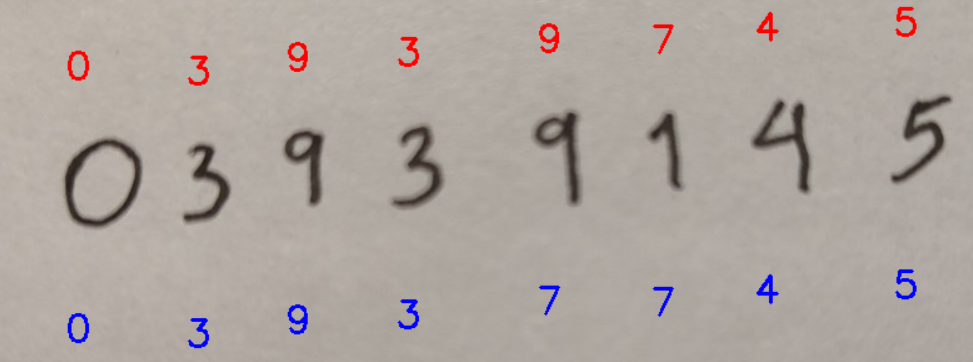
\includegraphics[width=\textwidth]{Image/test1.png}

    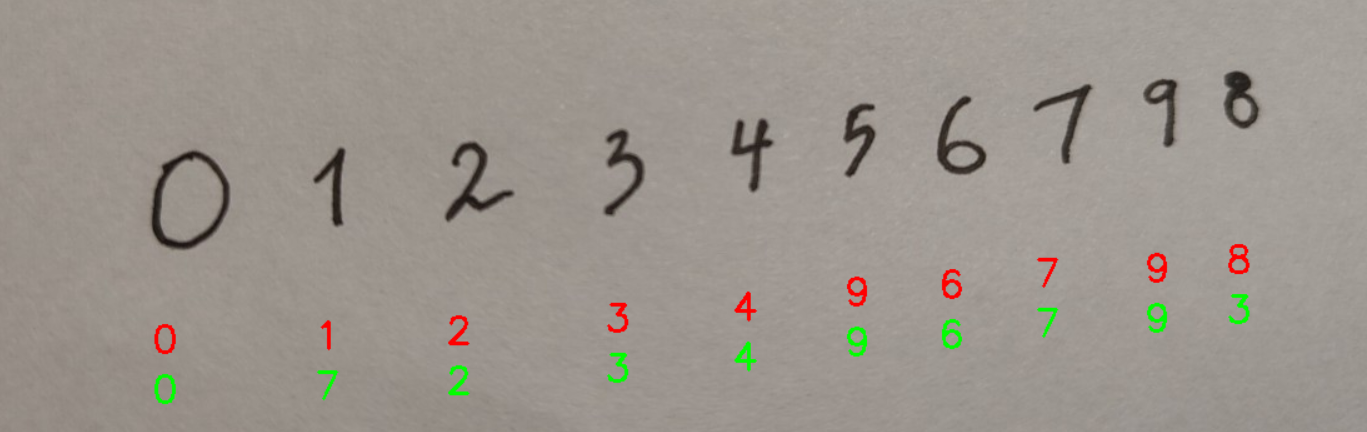
\includegraphics[width=\textwidth]{Image/test2.png}
    \caption{Kết quả dự đoán}
    \label{fig 2.8:Kết quả dự đoán}
\end{figure}

Từ hình 2.8 ta thấy. Ở bức ảnh phía trên, khi các chữ số được viết khá rõ ràng thì cả hai mô hình đều đưa ra dự đoán sai 1 chữ số.
Tuy nhiên ở hình dưới, khi các chữ số bị viết xấu hơn, các nét viết nguệch ngoạc thì mô hình Adversarial-regularized chỉ dự đoán sai 1/10 chữ số, trong khi mô hình cơ bản dự đoán sai 3/10 chữ số.
Từ đó ta thấy rằng, mô hình Adversarial-regularized có độ chính xác cao hơn và hoạt động tốt hơn mô hình cơ bản khi dữ liệu bị nhiễu. Và đây là một trong những ưu điểm của mô hình Adversarial-regularized.



\chapter{Kết luận} % Tên của chương

\label{Chapter3} % Thay X bằng số chương tương ứng; để trích dẫn chương này ở chỗ nào đó trong bài, hãy sử dụng lệnh \ref{ChapterX} 

Qua các chương trên chúng ta đã có cái nhìn tổng quan về TensorFlow, Neural Structured Learning. Chúng ta đã cài đặt và sử dụng  Neural Structured Learning
để xử lý bài toán phân loại chữ số viết tay. Chúng ta biết rằng Neural Structured Learning được khái quát hóa bằng hai phần chính là Neural Graph Learning và
Adversarial Learning tuy nhiên ở chương 2 chúng ta mới chỉ sử dụng Adversarial Learning để thử nghiệm, quan sát và đánh giá nó. Và ở mục 2.2 chúng ta đã minh chứng 
rằng Neural Structured Learning có thể giúp cải thiện độ chính xác của mô hình và giúp các mô hình hoạt động tốt hơn trên những tập dữ liệu kém.

Ở mục 1.1.2 chúng ta thấy rằng chỉ cần thêm một nhiễu rất nhỏ mà mắt thường không thể phát hiện được, ngay lập tức đã đánh lừa được mô hình cơ bản phán đoán sai.
Điều này mang lại nhiều nguy cơ cho các hệ thống sử dụng mạng neural để phát hiện, phân loại hình ảnh như camera an ninh hay xe tự lái vì chỉ cần các bức ảnh mà camera
thu thập được không đủ tốt hoặc có nhiễu thì sẽ gây ra sai lầm cho các phán đoán cho hệ thống. Đặc biệt là một số kẻ xấu có thể lợi dụng điều này để tấn công vào các hệ thống an ninh sử dụng
camera và thực hiện các hành vi của mình. Vì vậy việc tìm ra các cách để cải thiện độ chính xác của mô hình trên các tập dữ liệu kém tương tự như Adversarial Learning là rất cần thiết. 
%\include{Chapters/Chapter5} 


%----------------------------------------------------------------------------------------
%	Phần 15: PHỤ LỤC (THESIS CONTENT - APPENDICES)
%----------------------------------------------------------------------------------------

\appendix % Nói với LaTeX rằng những chương về sau được tính là phụ lục

% Hãy thêm những phụ lục (appendix) của khóa luận/tiểu luận vào thư mục Appendices
% Hãy bỏ chú thích những dòng nếu bạn đã bổ sung những phụ lục vào

%% Phụ lục A

\chapter{Các câu hỏi thường gặp} % Tên của phụ lục

\label{AppendixA} % Để trích dẫn chương này ở chỗ nào đó trong bài, hãy sử dụng lệnh \ref{AppendixA} 

%----------------------------------------------------------------------------------------

\section{Làm sao để thay đổi màu của đường dẫn liên kết?}

Màu sắc của đường dẫn có thể được thay đổi bằng các lệnh sau:

{\small\verb!\hypersetup{urlcolor=red}!}, hoặc

{\small\verb!\hypersetup{citecolor=green}!}, hoặc

{\small\verb!\hypersetup{allcolor=blue}!}.

\noindent Nếu bạn muốn ẩn toàn bộ đường dẫn, bạn có thể dùng lệnh:

{\small\verb!\hypersetup{allcolors=.}!}, hoặc thậm chí tốt hơn: 

{\small\verb!\hypersetup{hidelinks}!}.

\noindent Nếu bạn muốn hiển thị đường dẫn có màu trên file PDF còn ở bản in ra thì không, hãy sử dụng:

{\small\verb!\hypersetup{colorlinks=false}!}.


%----------------------------------------------------------------------------------------

\section{Làm sao để biểu diễn một bảng số liệu dài (hơn 1 trang), hoặc một bảng quá to?}

Thay vì sử dụng lệnh {\small\verb!\begin{table}!}, bạn hãy sử dụng lệnh {\small\verb!\begin{longtable}!}. Gói bổ trợ \code{longtable} (đã có sẵn trong template này) sẽ tự động giúp bạn ngắt bảng tại một vị trí khi bảng đã quá dài và biểu diễn phần còn lại của bảng ở những trang tiếp theo. Tài liệu về \code{longtable} bạn có thể tham khảo tại \href{https://mirror.kku.ac.th/CTAN/macros/latex/required/tools/longtable.pdf}{đường dẫn này}.

Trong trường hợp bảng số liệu dài theo bề ngang, bạn có thể xem xét phương án biểu diễn bảng số liệu theo chiều ngang của trang giấy như ví dụ Bảng~\ref{tab:treatments2} dưới đây. Để thực hiện cách này, bạn khai báo bảng như bình thường, rồi thay lệnh {\small\verb!\begin{table}!} bằng lệnh {\small\verb!\begin{sidewaystable}!}. Gói bổ trợ cho lệnh này đã có sẵn trong template này.

\begin{sidewaystable}
	\caption{Ảnh hưởng của phương pháp điều trị X và Y đối với bốn nhóm được nghiên cứu.}
	\label{tab:treatments2}
	\centering
	\begin{tabular}{l l l}
		\toprule
		\tabhead{Nhóm} & \tabhead{Phương pháp X} & \tabhead{Phương pháp Y} \\
		\midrule
		1	& 0.20	& 0.80	\\
		2	& 0.17	& 0.70	\\
		3	& 0.24	& 0.75	\\
		4	& 0.68	& 0.30	\\
		\bottomrule	\\
	\end{tabular}
\end{sidewaystable}


%----------------------------------------------------------------------------------------

\section{Làm sao để tìm đoạn code dưới định dạng bibtex cho tài liệu trích dẫn một cách hiệu quả?}

Bạn có thể tham khảo một số cách sau đây:

\begin{itemize}
	\item Cách 1: Sử dụng trang \href{https://scholar.google.com}{scholar.google.com}\\
	Bạn sẽ cần đi đến trang \href{https://scholar.google.com}{scholar.google.com} và hãy dán chính xác tên bài báo bạn muốn tìm kiếm. Sau đó bạn sẽ thấy một danh sách rất nhiều các đường dẫn đến bài báo và cả các bài báo tương tự mà bạn tìm kiếm. Hãy click vào biểu tượng: \textcolor{blue}{\faQuoteRight\;Cite}, rồi chọn tùy chọn \option{BibTeX} và bạn sẽ thấy đoạn code bạn cần.
	\item Cách 2: Sử dụng trang \href{https://www.researchgate.net/search}{researchgate.net}\\
	Bạn sẽ cần đi đến trang \href{https://www.researchgate.net/search}{researchgate.net} và hãy dán chính xác tên bài báo bạn muốn tìm kiếm. Sau đó bạn sẽ thấy một danh sách rất nhiều các đường dẫn đến bài báo và cả các bài báo tương tự mà bạn tìm kiếm. Hãy click vào tên bài báo phù hợp, sau đó click vào \option{Download citation}, rồi chọn tùy chọn \option{BibTeX} và \option{Citation only}. Để thuận tiện, bạn không cần download file chứa nội dung BibTeX về mà chỉ đơn giản chọn \option{Copy to clipboard} rồi dán nội dung vừa copy vào file \file{main.bib} của mình.
	\item Cách 3: Nếu một số tài liệu không xuất hiện ở cả hai trang phía trên, những tài liệu này thường là phần mềm hoặc kỉ yếu hoặc sách. Đối với phần mềm hoặc kỉ yếu, bạn có thể đi đến trang web chính thức chứa phần mềm hoặc kỉ yếu đó, nhiều khả năng là trang web sẽ hỗ trợ bạn trong việc trích dẫn. Đối với sách, bạn có nên tự xây dựng đoạn code BibTeX dựa trên một số đoạn code tương tự rồi thay đổi nội dung như số chương, số trang bạn đang muốn trích dẫn tới sao cho phù hợp.
\end{itemize}







%% Phụ lục B

\chapter{Liệt kê source code} % Tên của phụ lục

\label{AppendixB} % Để trích dẫn chương này ở chỗ nào đó trong bài, hãy sử dụng lệnh \ref{AppendixB} 

%----------------------------------------------------------------------------------------

\section{Ví dụ liệt kê code ngôn ngữ C/C++}

Code tính khoảng thời gian giữa hai thời điểm cho trước. Lệnh thực hiện là:
\begin{Verbatim}
\lstinputlisting{"Code/TimeDiff.cpp"}
\end{Verbatim}

File \file{TimeDiff.cpp}:
%https://www.programiz.com/cpp-programming/examples/time-structure
\lstinputlisting{"Code/TimeDiff.cpp"}


%----------------------------------------------------------------------------------------

\section{Ví dụ liệt kê thông tin ở terminal (console/command prompt) từ file text}

Sau khi biên dịch và chạy file \file{TimeDiff.cpp}, kết quả chạy được hiển thị ở terminal. Trong trường hợp bạn muốn liệt kê quá trình chạy, bạn có thể copy đoạn text ở terminal vào một file text, và liệt kê chúng chẳng hạn như:
\begin{Verbatim}
\lstinputlisting[style=console]{"Code/TimeDiff.txt"}
\end{Verbatim}

File \file{TimeDiff.txt}:
\lstinputlisting[style=console]{"Code/TimeDiff.txt"}


%----------------------------------------------------------------------------------------

\section{Ví dụ liệt kê code ngôn ngữ Python}

Code tính mã hash của một file. Lệnh thực hiện là:
\begin{Verbatim}
\lstinputlisting[style=codePython]{"Code/Hash.py"}
\end{Verbatim}

File \file{Hash.py}:
%https://www.programiz.com/python-programming/examples/hash-file
\lstinputlisting[style=codePython]{"Code/Hash.py"}


%----------------------------------------------------------------------------------------

\section{Ví dụ liệt kê code ngôn ngữ Matlab}

Code biểu diễn bản chất và sai số của phương pháp Euler và Heun trong việc giải phương trình vi phân. Lệnh thực hiện là:
\begin{Verbatim}
\lstinputlisting[style=codeMatlab]{"Code/EulerVisualization.m"}
\end{Verbatim}

File \file{EulerVisualization.m}:
\lstinputlisting[style=codeMatlab]{"Code/EulerVisualization.m"}


%----------------------------------------------------------------------------------------

\section{Ví dụ liệt kê file text thông thường (plain text)}

Một file text lưu giữ thông số của một lần chạy mô phỏng động học phân tử. Lệnh thực hiện là:
\begin{Verbatim}
\lstinputlisting[style=plaintext]{"Code/minim.mdp"}
\end{Verbatim}

File \file{minim.mdp}:
\lstinputlisting[style=plaintext]{"Code/minim.mdp"}




%\include{Appendices/AppendixC}


%----------------------------------------------------------------------------------------
%	(KHÔNG CHỈNH SỬA PHẦN NÀY)
%
%	Phần 16: TÀI LIỆU THAM KHẢO
%----------------------------------------------------------------------------------------

\begin{spacing}{1.15}
	\printbibliography[heading=bibintoc, title=Tài liệu tham khảo] % In ra tài liệu tham khảo
\end{spacing}

%----------------------------------------------------------------------------------------

\end{document}  
